\documentclass[oneside,10pt,a4paper]{report}
\usepackage[a4paper, left=3cm, right=3cm, top=3cm, bottom=3cm, headsep=10mm, footskip=12mm]{geometry}
\usepackage[T1]{fontenc}
\usepackage[ngerman, english]{babel}    % mehrsprachiger Textsatz
% babel: letzte Sprache in Optionen zeigt die Sprache des Dokumentes
% und kann durch den Befehl \selectlanguage{} geaendert werden
% Passen Sie die Optionen des babel-Paketes nach Bedarf an!
\usepackage{float}
\usepackage{graphicx}
\usepackage{url}
\usepackage{pdflscape}
\usepackage{mathtools}
\usepackage{amssymb, amsmath, amstext}
\usepackage{amsthm}
\usepackage{xcolor}
\usepackage{nameref}
\usepackage{siunitx}
\usepackage{makecell}
\usepackage{hyperref}
\usepackage{enumitem}
\usepackage[superscript,biblabel]{cite}
\usepackage{caption}
\usepackage{subcaption}
\usepackage{tabularx} 			% Tabellen erzeugen
\usepackage{multirow}			 % Zeilen in Tabellenbearbeitung
\usepackage{multicol} 			% Spalten in Tabellenbearbeitung 
\usepackage{lmodern}                        % Ersatz fuer Computer Modern-Schriften 
\usepackage{amsmath}                                           % zum besseren Aussehen am Bildschirm
\usepackage{booktabs} % für schönere Tabellen
\usepackage{sidecap}
\usepackage{rotating} % für die Landscape-Umgebung
\usepackage{afterpage}
\definecolor{Bluetitle}{HTML}{1F3864}
\definecolor{softbluetitle}{HTML}{274D7E}
\definecolor{Greyish}{HTML}{5A5A5A}
%\renewcommand{\refname}{Reference}
\usepackage{array,multirow}
\newcommand{\specialcell}[2][c]{%
	\begin{tabular}[#1]{@{}c@{}}#2\end{tabular}}
\usepackage{titlesec}

\titleformat{\chapter}[display]
{\normalfont\bfseries}{}{0pt}{\Huge}

\usepackage{lipsum} 


\begin{document}
	
	\begin{titlepage}
		\begin{center}
			\begin{figure}[h!tbp]
				
\includegraphics[width=\linewidth]{HUlogo.PNG}
			\end{figure}
			\vspace*{2 cm}
			
			\textcolor{Bluetitle}{\textbf{\huge Parasitologie - Praktikum}}\par
			
			\vspace*{2cm}
			\textcolor{Greyish}{\textbf{Versuchsdurchführende}}\par
			\textcolor{Greyish}{Huyen Anh Nguyen (572309)}\par

			\vspace*{0.5cm}
			\textcolor{Greyish}{\textbf{Versuchsort}}\par
			\textcolor{Greyish}{Haus 14, Kursraum}\par
			\textcolor{Greyish}{Gruppe 4}\par

			
			\vspace*{2 cm}
			\textcolor{Greyish}{\textbf{Versuchsleiter}}\par
			\textcolor{Greyish}{Prof. Dr. Kai Matuschewski}\par
			\vspace*{0.5cm}
			\textcolor{Greyish}{\textbf{Versuchsbetreuer}}\par
			\textcolor{Greyish}{Dr. Alexander Maier (ANU)}\par
			\textcolor{Greyish}{Linnea Polito}\par
			\textcolor{Greyish}{Grit Meusel}\par
			\textcolor{Greyish}{Dr. Richard Lucius}\par
			\textcolor{Greyish}{Peer Martin}\par
			\textcolor{Greyish}{Manuel Rauch}\par
			\textcolor{Greyish}{Dr. Katja Müller}\par

			\vspace*{2 cm}
			\textcolor{Greyish}{Abgabe 14. August 2024}\par
			
			
			
		\end{center}
	\end{titlepage}

	
	\tableofcontents
	\chapter{Note from the Author}
	Das Protokoll ist eine Collection von Einzelprotokolle der Versuchen, die in den Parasitologiepraktikum durchgeführt wurde.\\
	Es wurden Methoden gezeigt, wie eine Spezies identifiziert, untersucht und dessen Verhalten analysiert werden kann.\\
	Aufgrund dieser Diversitäten an Versuchen, wird das Protokoll in drei Großkapiteln unterteilt. Ich fand es sinnvoll die Kapiteln nach der Gattung der Tiere zu unterteilen, die wir in den Praktikum behandelt haben.\\
	Einige Bilder die hier verwendet wurde, wurden von Kommilitonen*innen aufgenommen und in einer WhatsApp-Gruppe annonym geteilt.\\
	\\
	Ich erkläre ausdrücklich, dass ich die Anmerkungen zur Anfertigung des Protokolls gelesen und befolgt habe, dass es sich bei der von mir eingereichte Arbeit um eine von mir erstmalig, selbstständig ohne fremde Hilfe verfasste Arbeit handelt und dass ich sämtliche verwendete zulässige Literatur (Fachpublikationen/-bücher), die unverändert oder abgewandelt wiedergeben werde, insbesondere Quellen für Texte, Grafiken, Tabellen und Bilder als solche kenntlich gemacht habe.\\
	Mir ist bewusst, dass Verstöße gegen diese Grundsätze als Täuschung betrachtet und entsprechend der Prüfungsordnung und/oder der Fächerübergreifenden Satzung zur REglung von Zulassung, Studium und Prüfung der Humboldt-Universität zu Berlin geahndet werden.
	
	
	\chapter{Hirudinea}	
	Hirudinea sind Egel die zu der Klasse Clitellata (Gürtelwürmer) gehören, wo auch die Regenwürmer dazu zählen. Ein apomorphes Merkmal der Clitellaten ist das sogenanntes Clitellum, (Das Epidermis ist verdickt und enthält viele Drüsenzellen, auch Drüsengürtel genannt), welches das Befruchtungsort für Eizelle und Spermazellen ist\cite{Kühkental}. Spezies der Clitellaten sind Hermaphroditen. \\
	Unter den Hirudinea gibt es räuberische (Haemopis sanguisuga), parasitische (Hirudo verbana) und aasfressende Arten, die aquatisch, amphibisch oder auch terrestrisch leben können.
	Die räuberische Arten ernähren sich von Wirbellosen, während die parasitische Arten von den Wirbellosen und Wirbeltieren sich ernähren. Bei den parasitären Arten werden meistens Wirte nicht spezifisch ausgesucht, solange die Wirte in der selben Klassenordnung stehen. \cite{Kühkental}.
	Aufgrund den fehlenden Gliedern bewegen sich die Hirudinea kriechend, schwimmend und raupenartig fort und nutzen dabei ihre Saugnapfen als Haftwerkzeug an Oberflächen und Bewegungshelfer.\\
	\\
	Ziel dieses Kapitels Hirudinea ist es, die Art eines unbekannten Egelspezies morphologische und genetische zu bestimmt. Eine morphologische Analyse kann mittels dichotomischen Bestimmungsschlüssel durchgeführt werden und eine genetische mittels DNA-Barcoding. Beide Methoden haben ihre Vor- und Nachteile, die hier behandelt werden.\\
	Zudem wird noch ein Vertreter der Hirudinea mit einem Vertreter der Schwestergruppe Oligochaeta (Wenigborster) verglichen.
	
	
		\section{Artenbestimmung mittels dichotomischen Bestimmungs- schlüssel}\label{Abschnitt: DichoBestim}
			\subsection{Einleitung}
				Der dichotomische Bestimmungschlüssel ist eine Methode, welches eine Spezies morphologisch und systematisch einen Reich, Stamm, Klasse, Ordnung, Gattung und Art anhand von bestimmten Entscheidungen zugeordnet wird.\\
				Das Wort dichotomie kommt aus den altgriechisch und bedeutet grob übersetzt "zweifacher Schnitt" \cite{wiki_dichotom}.
				Der Dichotome Bestimmungsschlüssel ist eine Tabelle oder Liste von Merkmalen, die für verschiedene Arten augelistet wurden. Dieser Bestimmungsschlüssel besitzt pro Merkmalskategorie zwei Merkmalsvarianten, wo der Nutzer entscheiden soll, welche der beiden Optionen zu der zu untersuchende Objekt passt. (Es gibt auch Submerkmalen unter den Hauptmerkmalen, um auch kleine Abweichungen abzudecken)\cite{dichotomer_schlüssel}. Durch die einzelnen Entscheidungen wird man zu einen Stamm, Klasse, Ordnung, Gattung oder Art geführt.\\

			\subsection{Methode}
				Unter einem Stereomikroskop wurde ein in Ethanol fixiertes Egelprobe (Körperlänge: 3 cm) untersucht.\\
				Die Merkmale wurden mit den dichotomischen Bestimmungsschlüssel "der Egel Deutschlands nach Clemens Großer" auf Moodle systematisch zugeordnet.\\
				Damit die Probe nicht austrocknet, wurde in regelmäßigen Abständen das Präparat mit Wasser befeuchtet.
			
			\subsection{Ergebnis}
			
				Für die Artenbestimmung wurde folgende Entscheidung getroffen:\\
				Augenzahl: 8 $\rightarrow$ 4 Augen in 1 vorderen Reihe, je 2 hinter liegenden, schräg gestellten Reihen (siehe Figure \ref{fig:feuchte_augen}) $\rightarrow$  Ordnung: Dina, Erpobdella, Trocheta $\rightarrow$ der gesamter Körper abgeplattet; alle Ringe gleichbreit $\rightarrow$  Gattung: Erpobdella $\rightarrow$  abgebrochen, aufgrund der knappen Zeit.\\
				\begin{figure}[H]
					\centering
					\begin{subfigure}[b]{0.55\textwidth}
						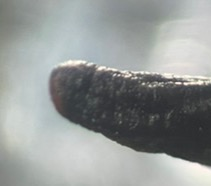
\includegraphics[width=\textwidth]{trockene_dichotom.jpg}
						\caption{Alte Egelprobe.}
						\label{fig: trockene_augen}
					\end{subfigure}
					\hfill
					\begin{subfigure}[b]{0.37\textwidth}
						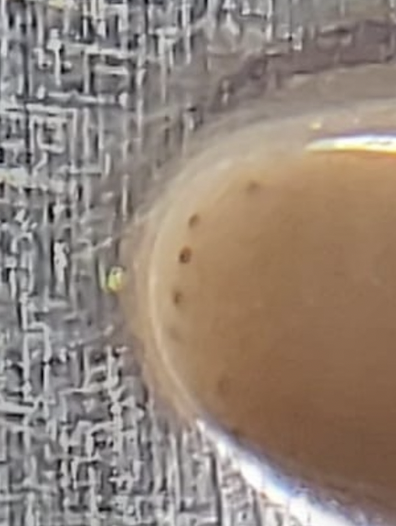
\includegraphics[width=\textwidth]{Dichotom_augen}
						\caption{Frische Egelprobe}
						\label{fig:feuchte_augen}
					\end{subfigure}
					\caption{20-fache Vergrößerung der vorderen Körperteil des Egels. Aufgrund des Zustandes des Präparates in \ref{fig: trockene_augen} wurde das Präparat \ref{fig:feuchte_augen} von einer Kommiliton*in  untersucht. Beide Spezies gehören zur selben Art. In \ref{fig:feuchte_augen} ist gut zu erkennen, dass der Egel 4 Augen ganz vorne nebeneinander gereiht besitzt und mindest ein Auge schrägstellt dahinter liegt.}
					\label{fig: Dicho_augent}
				\end{figure}
			
			
			\subsection{Diskussion}
				Anhand des dichotomischen Bestimmungsschlüssel wurde das Egelpräparat zu der Gattung Erpobdella zugeordnet.
				Da der Versuch nachmittags durchgeführt wurde und die Präparate auch vormittags verwendet wurde, war der Zustand des Egels nicht mehr optimal für eine ordentliche Bestimmung.
				Die Verwendung des dichotomischen Bestimmungsschlüssel erwies sich für Amateuere als schwierig, da viele Merkmale uneindeutig zugeordnet werden kann, insbesondere wenn das Präparat nicht in optimalen Konditionen vorliegt.\\
				Ein Vorteil dieser Methode ist, dass es schnell und kostengünstig durchführbar ist.\\
				Da hier aufgrund von Zeitmangel nicht möglich war die Art zu bestimmen, wird diese mit der DNA-Barcoding durchgeführt.
		
		\section{Artenbestimmung mittels DNA-Barcoding}
			\subsection{Einleitung}
				Die DNA-Barcoding ist eine Methode, weches mit der Genomensequenz, die Art bestimmt werden kann.
				Da jede Art eine einzigartige genetische Sequenzabfolge besitzt, eignet sich diese Methode bestens eine Spezies phylogenetisch zu analysieren\cite{Folmer} \cite{Herbert}.\\
				Hierfür werden Gensequenzen, sogenannte Markergens, der Spezies untersucht, die innerhalb der Art konserviert bleiben.
				Die erhaltende Sequenz wird dann mit der Datenbank verglichen und nach Übereinstimmungen überprüft. Diese Methode setzt vorraus, dass die Gensequenz auch in der Datenbank archiviert wurde.\\
				Für Hirudinea Proben wird als Sequenzmarker häufig das  Cytochrome C Oxidase subunit 1 Enzym (abgekürzt: COI), ein Gen in den Mitochondrien, verwendet\cite{Folmer}. Mitochondrialer DNA besitzen keine Introns und wird maternal haploid vererbt, so dass es nicht wie beim Kerngenom zwei verschiedene Varianten eines Gens existieren.\\
				\\
				Damit für die Sequenzierung genug DNA-Material zur Verfügung stehen, wird hier die Polymerase Chain Reaction-Methode (abgekürzt: PCR) verwendet.\\
				Das Verfahren ermöglich das der gewünschten Genabschnitt schnell und in hohen Konzentration zu vervielfachen.
				Für die PCR wird ein hitzestabiles DNA-Polymerase I-Enzym (hier Taq-Polymerase aus dem Thermus aquaticus-Bekterium) benötigt, da für die Annealing die doppelsträngige DNA durch Hitze zu Einzelstränge aufgeschmolzen wird.
				Für die Amplifikation benötigt die Taq-Polymerase Primers, um an die DNA zu binden. Der Primer sollte da binden, so dass bei der Amplifikation die Gen-Sequenz des CytochromeC Oxidase mit amplifiziert wird.
				Hier wird der Forward-Primer LCO1490 (bindet am Nicht-codogener Strang) und Reverse Primer HC02198 (bindet am Codogener Strang) von Folmer (1994) verwendet (siehe Table \ref{tab: Primer}), welches ermöglicht ein 659bp langes Genfragmentes des COI-Gens zu amplifizieren.\\
				Im Anschluss wird mittels einer Agarosegelelektrophorese die Fragmente nach der Größe aufgetrennt und sequenziert.\\
				
			
			\subsection{Methode}
				\textit{14. Juni 2024}\\
				\\
				Für die gDNA-Isolierung wurde das Genomic DNA tissue kit verwendet.\\
				Ein grobes Egelgewebestück (circa 20 mg) wurde mit einem Skalpell zerkleinert und mit 400 $\mu$L Lysispuffer und 25 $\mu$L Proteinase K für 30 Minuten bei 56°C unterm Schütteln inkubiert. Dann wurden 250 $\mu$L Bindingsolution SBS zugegeben und auf einem Spinfilter überführt. Diese wurde für 2 Minuten bei 10000 x g zentrifugiert und das Filtrat verworfen.\\
				600 $\mu$L Waschpuffer wurde dann auf den Spinfilter pipettiert und für 1 Minute für 11000 x g zentrifugiert. Dieser Schritt wurde mit 300 $\mu$L Waschpuffer wiederholt. Am Ende wurde die Probe auf maximalen Speed für 30 Sekunden abzentrifugiert.\\
				Der Spinfilter wurde auf einem 1.5 mL Eppendorf-Röhrchen gesteckt. Auf dem Filter wurde 50 $\mu$L RNase freies Wasser pipettiert und mit geöffneten Deckel bei 11000 x g für 2 Minuten zentrifugiert.
				\\
				\textit{12. Juli 2024}\\
				\\
				Die Konzentration vom gDNA wurde photometrische bestimmt und beträgt 15.2 mg/mL (wurde von Grit Meusel durchgeführt).
				Es wurden 2 $\mu$L gDNA mit 23 $\mu$L Mastermix pipettiert. Das gleiche wurde auch mit der Negativkontrolle (Wasser) wiederholt(Pipettierschema für den Mastermix siehe Table \ref{tab: Mastermix-Pipettierschema}).
				Die Proben werden dann für 34 Cyclen amplifiziert (PCR-Cyclen siehe Table \ref{tab: PCR-Cyclen}).
				\\
				\textit{14. Juni 2024}\\
				\\
				5 $\mu$L amplfizierte PCR-Proben wird mit 1 $\mu$L 6x Gel-Puffer vermischt und auf einem 1$\%$igen Agarosegel aufgetragen. Zusätzlich wird ein DNA Marker mitraufpipettiert für die Größenbestimmung.
				Der Gellauf lief bei 100V für 1 Stunde und das Geld wurde unter ultravioletes Licht analysiert. Die Sequenzbestimmung wird von den Versuchsbetreuer durchgeführt.\\
				\\
				Die Sequenzabfolge wird mit der National Library of Medicine-Datenbank abgeglichen und ein Alignment-Tree in MegaX erstellt.
				
			
			\subsection{Ergebnis}
				Der Gellauf zeigt eine bei der Probe-Spur eine Bande bei circa 600bp und bei der Negativkontrolle -Spur keine Banden.
				
				\begin{figure}[H]
					\centering
					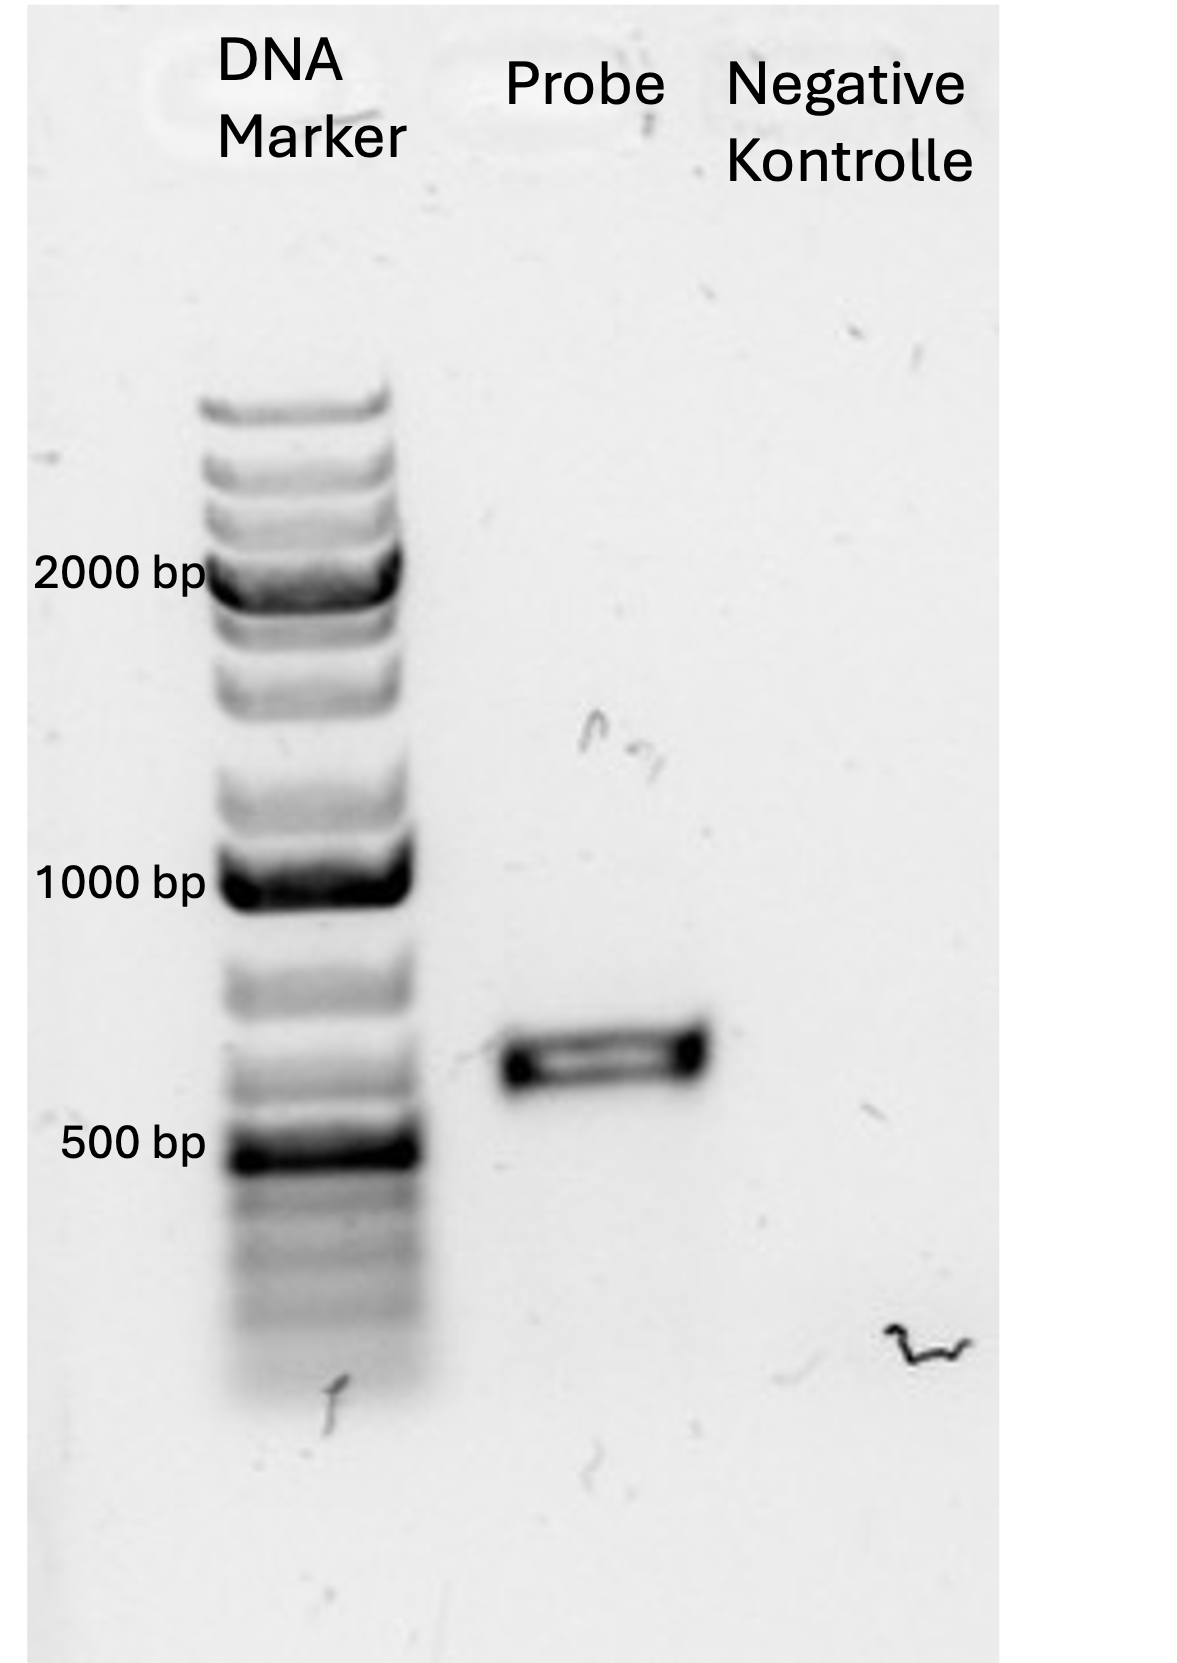
\includegraphics[scale=0.7]{gel.png}
					\caption{Größenauftrennung der gDNA PCR-Probe von der unbekannte Egelgewebestücks und der Negativkontrolle (Wasser) aufgetrennt auf einer 1$\%$-Agarosegel, mit einem DNA-Marker als Größenvergleich. Die Banden wurde mit ultraviolettes Licht sichtbar gemacht. In der Probe-Spur ist eine Bande bei 600bp sichtbar.}
					\label{fig:Agarosegel}
				\end{figure}
				
				\begin{table}[H]
					\centering
					\caption{Consensus-Sequenz Gruppen 1-7. Die Bande im Bereich 600 bp wurde aus der Agarosegelelektrophorese isoliert und sequenziert.}
					\label{tab: Consensus-Sequenz Gruppen 1-7}
					\begin{tabular}{l}
						TTTATTCTAGGAAGCATGGGTCAGCTATAGCTGGCACAGGCATAAGGGTACTAATTCGAA\\
						TTGAGTTAGCCCAACCTGGCACATTTTTAGGAAACGATCAAATTTATAACACTATTGTAA\\
						CCGCTCACGGGCTAGTAATAATTTTCTTTATAGTAATACCTATTTTAATTGGAGGATTTG\\
						GAAATTGGTTGATTCCATTAATAATTGGTGCACCAGATATAGCCTTTCCTCGACTCAATA\\
						ATCTAAGATTTTGACTATTACCCCCATCAATAATTATATTAGTCTTCTCTGCATTTGTAG\\
						AAAATGGTGTGGGTACTGGATGAACAGTATACCCTCCCTTAGCATATAATATTGCCCACT\\
						CTGGCCCATCAGTAGATATGGCTATTTTCTCATTACATTTAGCAGGAGCTTCATCTATTT\\
						TAGGATCATTAAACTTTATTTCCACTGTAGCAAATATACGATGAAAAGGTATATCATTAG\\
						ATCGAATCCCTTTATTTATTTGATCAGTAATTATTACTACAGTACTTCTACTTCTATCAT\\
						TACCAGTTTTAGCAGCTGCCATTACTATATTACTGACTGATCGAAACTTAAATACATCCT\\
						TCTTTGACCCTGCAGGAGGAGGAGACCCAATCCTATTCCAACATTTATTTTGATTTTTTG\\
						GTCACC\\
					\end{tabular}
				\end{table}
				
				In Table \ref{tab: Consensus-Sequenz Gruppen 1-7} wurde die Sequenz der isolierte Probebande dargestellt.
				Mit der Datenbank glich die sequenzierte COI-Sequenz mit 99.49$\%$ mit der Art Erpobdella octoculata zusammen. Die Referenzsequenz (siehe Table \ref{tab: Vergleichssequenz}) zeigt mit der Art Erpobdella testacea eine Übereinstimmung von 99.69$\%$.\\
				Beide Sequencen murden mit der MUSCLE Alignment-Algorithmus ausgewertet und zeigen 266 gemeinsame BAsenpaare auf.
				In Figure \ref{fig: Baum} wurden die beiden Erpobdellaarten mit 9 weiteren Arten, die aus den Abschnitt \ref{Abschnitt: DichoBestim} erwähnte dichotome Bestimmungsschlüssel ausgewählt wurden, in Relation gestellt und mit der Maximum Parsimony Algorithmus den Verwandschaftsgrad bestimmt. In Figure \ref{fig: Baum} stehen die beiden Erpobdella-Arten nicht gegenüber.
				
				\begin{figure}[H]
					\centering
					\includegraphics[scale=0.7]{Anhs Tree.png}
					\caption{Aligmenttree mit 11 Arten. Es wurde nach dem MUSCLE-Algorithmus alignt und ein Alignmentbaum nach dem Maximium Parsimony Methode erstellt. Die Spezies die in den Kurs untersucht wurde trifft mit 99.49 $\%$ dem Erpobdella octoculata zu. Die Verwandschaftsbeziehung zu Erpobdella testacea, welches die Referenzsequenz vom Betreuer zur Verfügung gestellt wurde zeigt, dass beide keine Schwesterngruppe bilden.}
					\label{fig: Baum}
				\end{figure}
				
			
			\subsection{Diskussion}
				Vom Egelgewebestück wurde eine Sequenz amplifiziert, dass 664bp lang ist (siehe Table \ref{tab: Consensus-Sequenz Gruppen 1-7}). Diese DNA-Fragment wurde in der Agarosegelelektrophorese auch in den Bandenbereich von circa 600bp aufgetrennt.\\
				Der Sequenzvergleich mit der Datenbank der National Library of Medicine wurde zeigte der Egel eine  Übereinstimmung von 99.49$\%$ mit der Art Eropbdella octoculata.  
				In Abschnitt \ref{Abschnitt: DichoBestim} wurde mittels dichotomisches Bestimmungsschlüssel ebenfalls morphologisch die Gattung Erpobdella dem Egel zugeordnet.\\
				Der bestimmte Egelart Eropbdella octuculata und Erpobdella testacea bilden keine monophyletische Gruppe, wenn andere Egelarten in Bezug genommen wird (siehe Figure \ref{fig: Baum}).\\
				Die Artenbestimmung mit der DNA-Barcoding ist deutlich kostspieliger und zeitaufwendiger als die Methode mit dem dichiotomischen Bestimmungsschlüssel. Mit beiden Methoden konnte die gleiche Gattung bestimmt werden.
				Für eine eindeutige Zuweisung der Art ist eine genetische Analyse jedoch unabdingbar.

				
		\section{Vergleich Hirudinea und Regenwurm}
			\subsection{Einleitung}
				In der Gruppe der Clitellata gehören die Oligochaeta (Wenigborster) und die Hirudinea (Egel), zu der großen Gruppen der Anneliden (Ringelwürmer).
				Oligochaeta ist nur ein Sammelbegriff für die paraphyletische Gruppe, die nicht monophyletisch sind. Aus den Oligochaeta wird hier der Regenwurm Lumbricus terrestris als Vertreter auserwählt. Lumbricus terrestris ist der bekannteste Regenwurmart in Europa und lebt in den Boden von Wiesen und Gärten \cite{regenwurm}. Sie gehören zu den Destruenten und tragen zum Ökosystem bei. Von den Hirudinea wird der medizinischer Egel Hirudo verbana als Vertreter genommen. Der Egel ist ein Ektoparasit, welches sich von Fischen, Amphibien und Wirbeltieren ernährt. Sie kommen in den Gewässern der Mittelmeerraum vor \cite{hirudo}. In der Medzinin  besitzen diese Tiere eine besondere Bedeutung, da ihr Speichel gerinnungshemmend, blutsenken, entzündungshemmend und lokal betäubend wirkt.\\
				In diesen Versuch werden von den beiden Arten die Körpersysteme morphologisch auf Unterschiede und Gemeinsamkeiten untersucht.\\
				
				
			\subsection{Methode}
				Der Hirudo verbana (Egel) wurde unter einem Stereo-Mikroskop präperiert und auf einem mit Alufoliebedeckten Styroformplatte fixiert. Entlang der Mittelline der Bauchseite wurde die Bauchseite mit der stumpfen Seite der Schere aufgeschnitten und fixiert. Der Verdauungstrakt wurde betrachtet und vorsichtig abgenommen, um den inneren Rückeninnenbereich, die Geschlechtsorganen und Harnsystem betrachten zu können. Das Nervensystem konnte nicht erkannt werden.\\
				Die Morphologie wurde dann mit den Regenwurm aus MB5 (Lumbricus terrestris) verglichen.
			\subsection{Ergebnis}
				
				In Table \ref{tab: Egel vs Regenwurm} sind die Merkmale von den Hirudo verbana und Lumbricus terrestris für die Organsysteme Verdauungs-, Kreislauf-, Nerven-, Harnsystem und Fortpflanzungsorgane aufgelistet. 
				\begin{table}[H]
					\centering
					\caption{Merkmale in den Organsysteme zwischen der Hirudo verbana (medizinischer Egel) und Lumbricus terrestris (Regenwurm). Die Merkmale sind in Figure \ref{fig:Egel_ana} (Hirudo verbana) und \ref{fig:Regenwurm_ana} (Lumbricus terrestris) graphisch dargestellt.}
					\label{tab: Egel vs Regenwurm}
					\begin{tabular}{c c c}
						\toprule
						& Hirudo verbana & Limbricus terrestris\\
						\midrule
						\multirow{7}{*}{\parbox[t]{2cm}{Verdauungs- system}} & \multirow{7}{*}{\parbox[t]{6cm}{Der Magen erstreckt sich über die Körperlänge, die sind in 10 Zweipaarige Blindsäcke(letztes Paar ist stark vergrößeret) auffächern. Am Kopfbereich befindet sich der Kiefern mit Zähnen aus Kalzit. Der Mund geht ins Pharynx über}}&\multirow{7}{*}{\parbox[t]{6cm}{Der obere Verdauungstrakt besteht aus dem Mund, Pharynx, Oesophagus und Kalksäckchen. Bevor es zu den Muskelmagen übergeht, ist da noch der Kropf. Der Magen ist nur zwei Körpersegmente lang und geht dann zu den Darmtraktes über}}\\
						&&\\
						&&\\
						&&\\
						&&\\
						&&\\
						&&\\
						\midrule
						\multirow{5}{*}{\parbox[t]{2cm}{Kreislauf- system}}& \multirow{5}{*}{\parbox[t]{6cm}{Lateralkanäle und Seitenkanäle durchziehen den Egel und in der Mitte des Körpers befindet sich das Dorsalgefäß}}&\multirow{5}{*}{\parbox[t]{6cm}{Das Rückengefäß liegt auf dem Darm und besitzt Gefäßschlingen, die das Blut zu den Bauchgefäß pumpt. Die Gefäßschlingen wird auch Lateralherz genannt}}\\	
						& &\\
						&&\\
						&&\\
						&&\\
						\midrule
						\multirow{2}{*}{\parbox[t]{2cm}{Nervensystem}} & \multirow{2}{*}{\parbox[t]{6cm}{ein Cerebralganglien unterhalb des Kiefers}}&\multirow{2}{*}{\parbox[t]{6cm}{zwei Cerebralganglien oberhalb des Pharynx}}\\
						& &\\
						\midrule
						\multirow{4}{*}{\parbox[t]{2cm}{Fort- pflanzungs- organe}} & \multirow{4}{*}{\parbox[t]{6cm}{Räumlich getrennte Geschlechtsorgane. Besitzt Vagina und eine Penistasche. Über den ganzen Körper sind die Hoden verteilt.}}&\multirow{4}{*}{\parbox[t]{6cm}{Weiblicher und Männliche Geschlechtsorgane sind räumlich voneinander getrennt, keine Vagina oder Penis.}}\\
						& &\\
						&&\\
						&&\\
						\midrule
						\multirow{2}{*}{\parbox[t]{2cm}{Harnsystem}}& \multirow{2}{*}{\parbox[t]{6cm}{Besitzen lateral paarige  Harnblasen mit Nephridien diein jeden Segment}}&\multirow{2}{*}{\parbox[t]{6cm}{Besitzen paarige Nephridienschlingen in jeden Segmenten}}\\
						& &\\
						\bottomrule
					\end{tabular}
				\end{table}
				
			\subsection{Diskussion}
				Hirudo verbana und Lumbricus terrestris zeigen einige gemeinsame Merkmale. So ist der Körper mit kräftigen Ring- und Längsmuskeln gekleidet und das Harnsystem tritt paarig in jeden Körper Segment auf (Ausgenommen der Kopfberech). Beide Arten besitzen weibliche und männliche Geschlechtsorgane, die räumlich durch Segmente getrennt sind, um Selbstbefruchtungen zu verhindern.\\
				Durch die verschiedene Ernährungsweisen vom Hirudo verbana und Lumbricus terrestris gibt es in den Verdauungssystem die größten Unterschiede. So hat der Egel aufgrund seines Lebensform einen stark vergrößerten Magen.\\
				Aufgrund des Lebensstils der Egel, kann dieser für eine sehr lange Periode ohne Nahrung auskommen. Wenn der Egel sich an einem Wirt mit den Zähnen festgebissen hat, saugt er sich mit Blut soweit voll, bis die Blindsäcke mit Blut gefüllt sind. Bei einem vollen Magen löst sich der Egel ab und beginnt mit der Fortpflanzung.\\
				Der Regenwurm hingegen ernährt sich von toten Pflanzenreste und benötigt ein starken muskulösen Magen, um zusammen mit den eingesaugten Sand diese zerkleinern zu können. Den zusätzlich Kalksäckchen, den der Regenwurm besitzt, spielt bei der Homöostase eine Rolle \cite{Kühkental}. 
				
	
	
	\chapter{Trematoden}
		Trematoden (Saugwürmer) gehören zu der Klasse der Plathelminthes (Plattwürmer) und bilden mit den Cestoda(Bandwürmer) eine monophyletische Gruppe.\\
		Die meisten Trematoden sind Endoparasitisch und nutzen Wirbellosen als Zwischenwirt und Wirbeltieren als Endwirt.\\
		Während des Entwicklungszyklus ist es für die Trematodenarten notwendig die Wirte zu wechseln, um auch von der asexuellen zu der sexuellen Phase wechseln zu können.
		Morphologisch besitzen die Trematoden am Mund und Bauch Saugapparate, mit denen sie sich an dem Wirt haften können. \\
		Bis auf die Schistosoma sind die Trematoden zwittrig.
		
		\section{Einleitung}
			Als Vertreter der Trematoden wird der kleine Leberegel Dicrocoelium dendriticum genommen.
			Während der Entwicklungsphase parasitiert der Dicrocoelium dendriticum zwei Zwischenwirte in der asexuellen Phase, bevor er im Endwirt in die sexuelle Phase übergeht.
			Die Eiern des Parasites wird von den Endwirt (welches meistens große Weidetiere sind) mit den Kot ausgeschieden. Der erste Zwischenwirt, die Landschnecke nimmt die Eier auf, wo die Larven schlüpfen. Dieses Larvenstadium wird auch Sporozytenstadium genannt, wo die Sporozyten in der Schnecke sich zu Zerkarien entwickelt, bevor diese den Wirt wechselt. Beim Wirtswechel sekretiert die Schnecke die Larven als mucöse Bälle ab, welches der zweite Zwischenwirt, die Ameise, dann frisst. In der Ameise wandert ein Zerkarien-Zelle in das Gehirn und steuert die Motorik der Ameise.
			Die Ameise wird so manipuliert, dass diese bei Nacht einen Grashalm hochklettert und dort solange verharrt, bis der Endwirt (beispielsweise die Kuh), das Gras mit der Ameise frisst.
			In dieser Zeit verbleiben die anderen Parasiten als Metazerkarien im Magen der Ameise.
			Im Magen des Endwirtes wird die Ameise mit der Zerkarie im Hirn verdaut, während die anderen Metazerkarien durch die Zystenhülle vor der Magensäure geschützt wird.
			Nach der Passage des Magens, wandern die Metazerkarien zu den Gallengängen und entwickeln sich zu den adulten Würmer.
			Als adulter Wurm beginnt dann die sexuelle Fortpflanzung, wo der Parasit die Eier in die Gallensäfte absondern. Der Gallensaft gelangt dann in den Darm und wird mit den Kot ausgeschieden.\\
			In diesen Versuch wird die Anatomie des kleinen Leberegelsund die Larvenstadien in der Schnecke untersucht.
			
			
		\section{Methode}
			\subsection{Malzacherfärbung}
			Die in 70$\%$ Ethanol fixierten adulten Dicrocoelium dendriticum wurden für 5 Minuten in Boraxcarmin fixiert.Für 1 Minute lang wird das Präparat in Leitungswasser differenziert bis das Gewebe zu rosa verblasste.\\
			Mit Strablaulösung 1$\%$ Astrablau, 3$\%$ Weinsäure in ddH$_2$O) wurde für 5 Minuten in gefärbt und anschließend für 2 Minuten in 3$\%$ Weinsäure solange entfärbt, bis das Gewebe rosa-lila wurde.
			Das Präperant wird in einer aufsteigende Alkoholreihe dehydriert (10 Minuten in 50$\%$ Ethanol, zwei Mal 10 Minuten 70$\%$, 10 Minuten in absoluten Ethanol und dann 5 Minuten zwischen zwei Objekträgern in absoluten Ethanol ). Als letzter Entwässerungsschrit wurde das Objekt für 5 Minuten in absoluten Ethanol gelegt.\\
			Vor dem Eindecken wurde das Objekt für 10 Mintuen in Wintergrünöl inkubiert.\\
			
			\subsection{Trematodenlarven in der Wasserschneckenleber}
				Mit einer Pinzette wird ein Stück infizierte Wasserschneckenleber in Wasser zerrupft. Ein Tropfen des zerrupften Lebergewebe wird unterm Mikroskop nach den Trematodenlarven untersucht.
				
		\section{Ergebnis}
			\subsection{Portrait des adultes Dicrocoelium dendriticum}
				\begin{figure}[H]
					\centering
					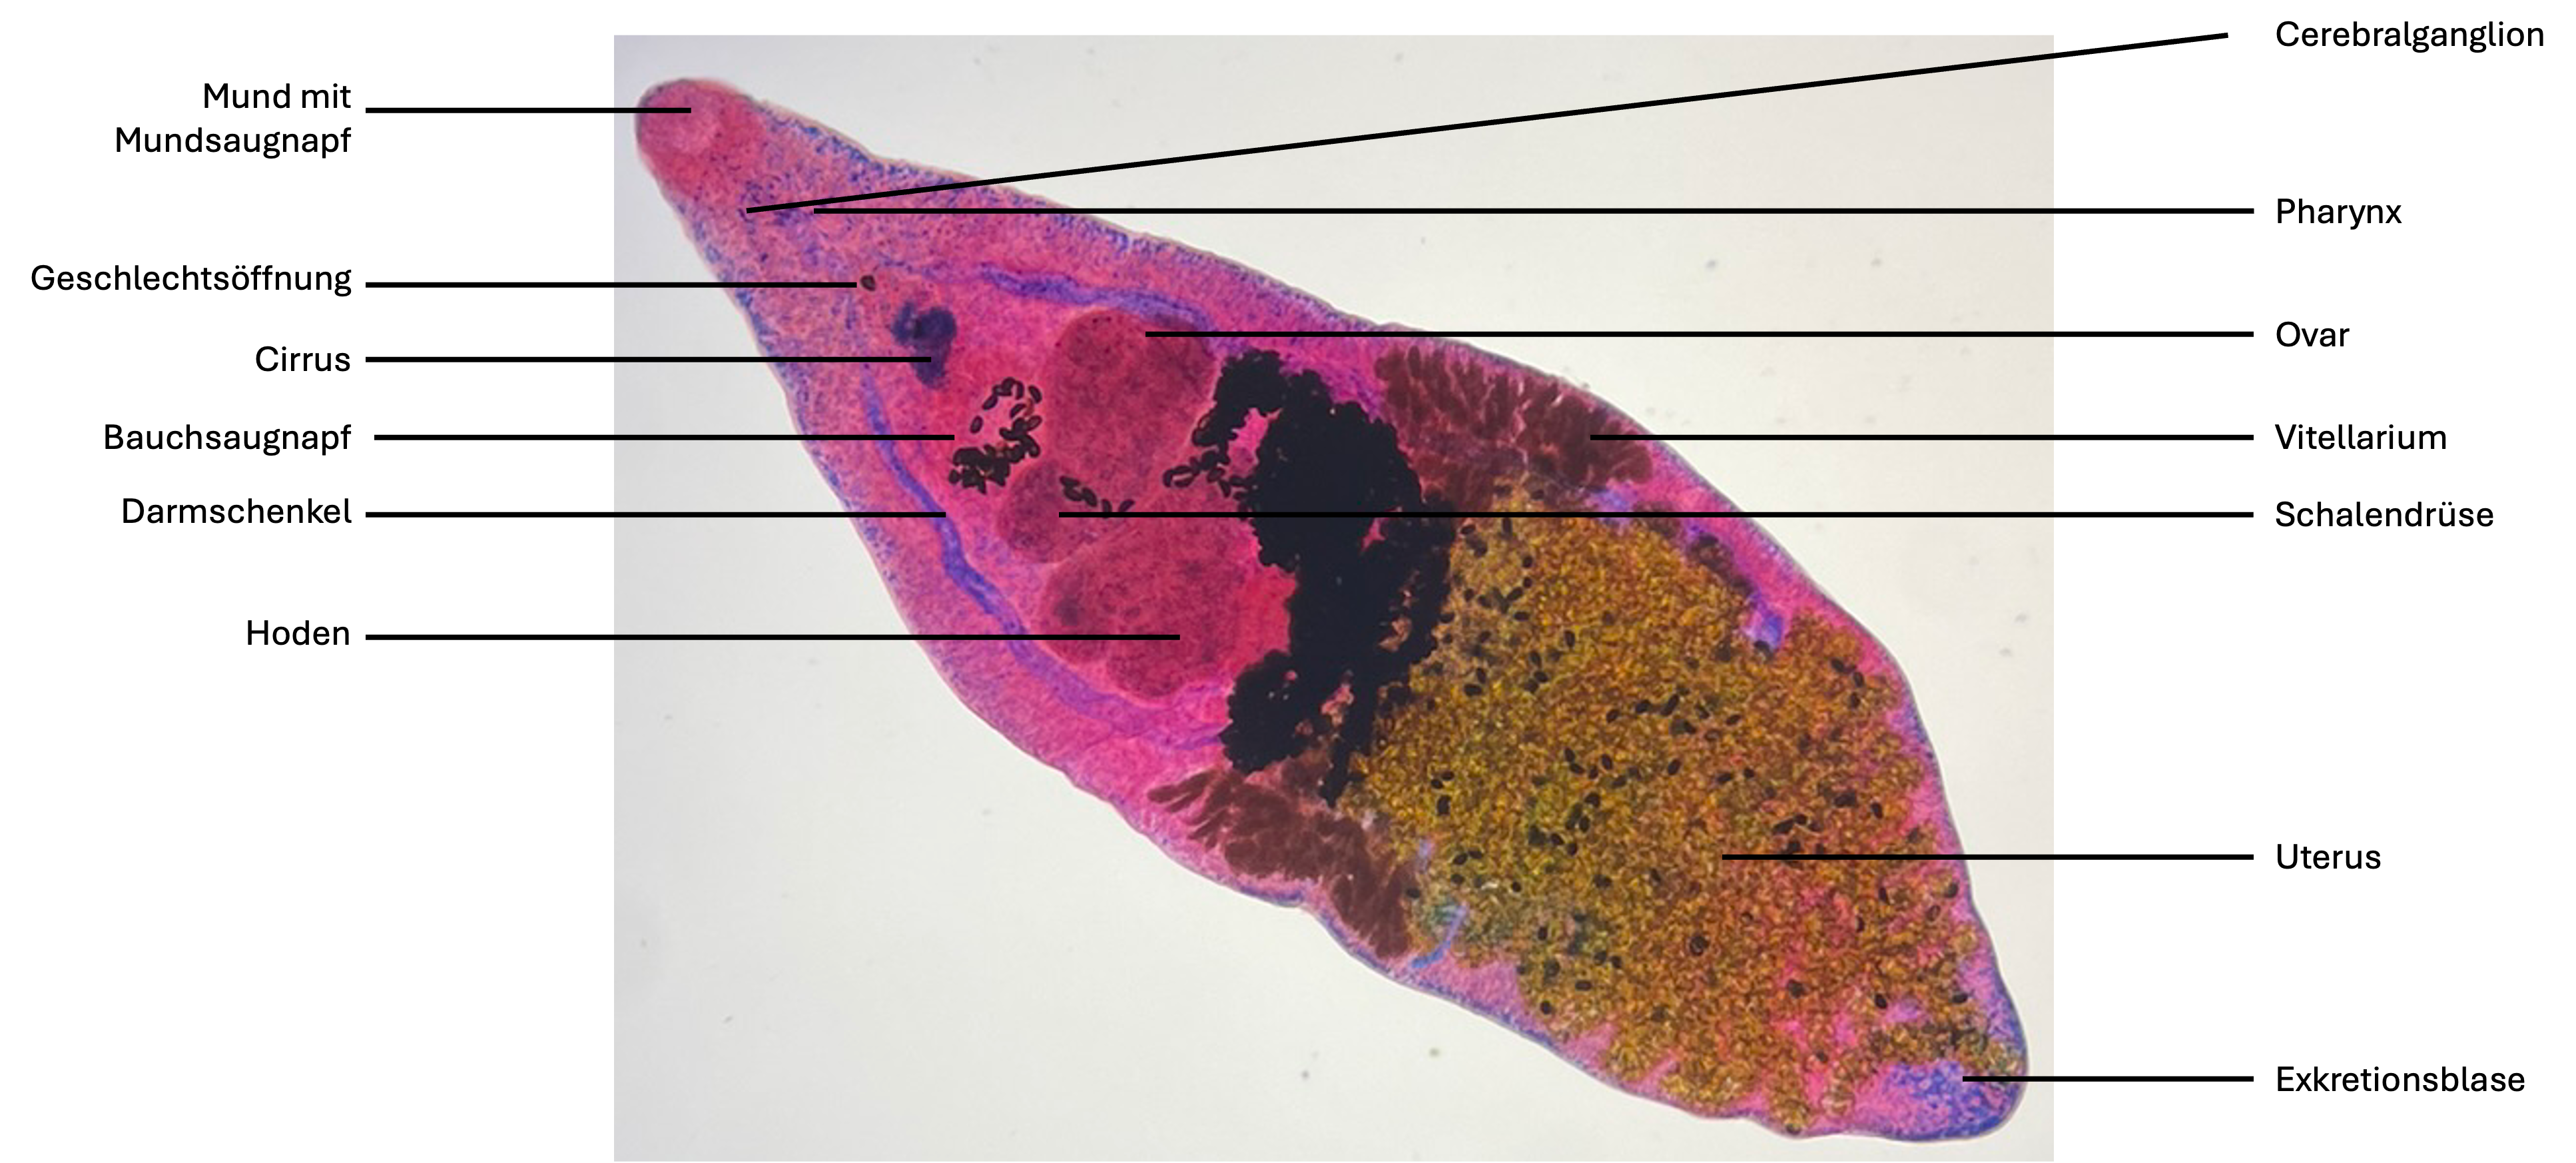
\includegraphics[scale=0.5]{Dicrocoelium dendriticum.png}
					\caption{40-fache Vergrößerung des adultes Dicrocoelium dendriticum (Leberegel) aus einer infizierten Wasserschneckenleber.}
					\label{fig: TrematodenMalzacherfärbung}
				\end{figure}
				
				Die adulte Dicrocoecoelium dendriticum besitzt zwei Saugnäpfe, eine am Mund und eine am Bauch. Nach dem Mund folgt das Pharynx, das in den gegabelten Darm hinübergeht. Wie in Figure \ref{fig: TrematodenMalzacherfärbung} zu sehen, nehmen die Geschlechtsorgane des Plattwurmes mehr als die Hälfte des Tieren ein. Der Uterus füllt mehr als die Hälfte des Volumen. Da die Art zwittrig ist, besitzt diese das weibliche und männliche Geschlechtsorgane. Das Cerebralganglion befindet sich unterhalb des Mundsaugnapfes. Das Cirrus befindet sich an den Geschlechtsöffnung.\\
				Die Exkrationsblase ist in den Präparat kaum zu erkennen, liegt jedoch am hinteren Ende des Wurmes.
				
			\subsection{Trematodenlarven}
				In Figure \ref{fig: Trematodenlarven} befindet sich zwei Trematodenlarven in zwei verschiedenen Larvenstadien in der Leber der Wasserschnecke, die Redie-Form (Figure \ref{fig:Redie}) und die Zerkarien in verschiedenen Formen (Figure \ref{fig: Zerkarien}).
				
				\begin{figure}[H]
					\centering
					\begin{subfigure}[b]{0.4\textwidth}
						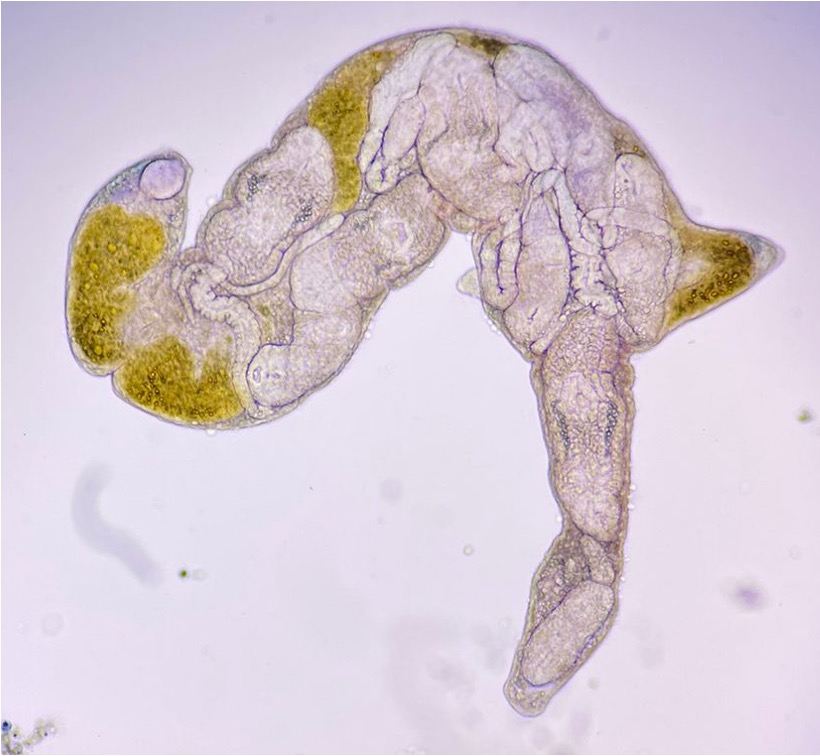
\includegraphics[width=\textwidth]{Redie.jpg}
						\caption{Redie-Form}
						\label{fig:Redie}
					\end{subfigure}
					\hfill
					\begin{subfigure}[b]{0.45\textwidth}
						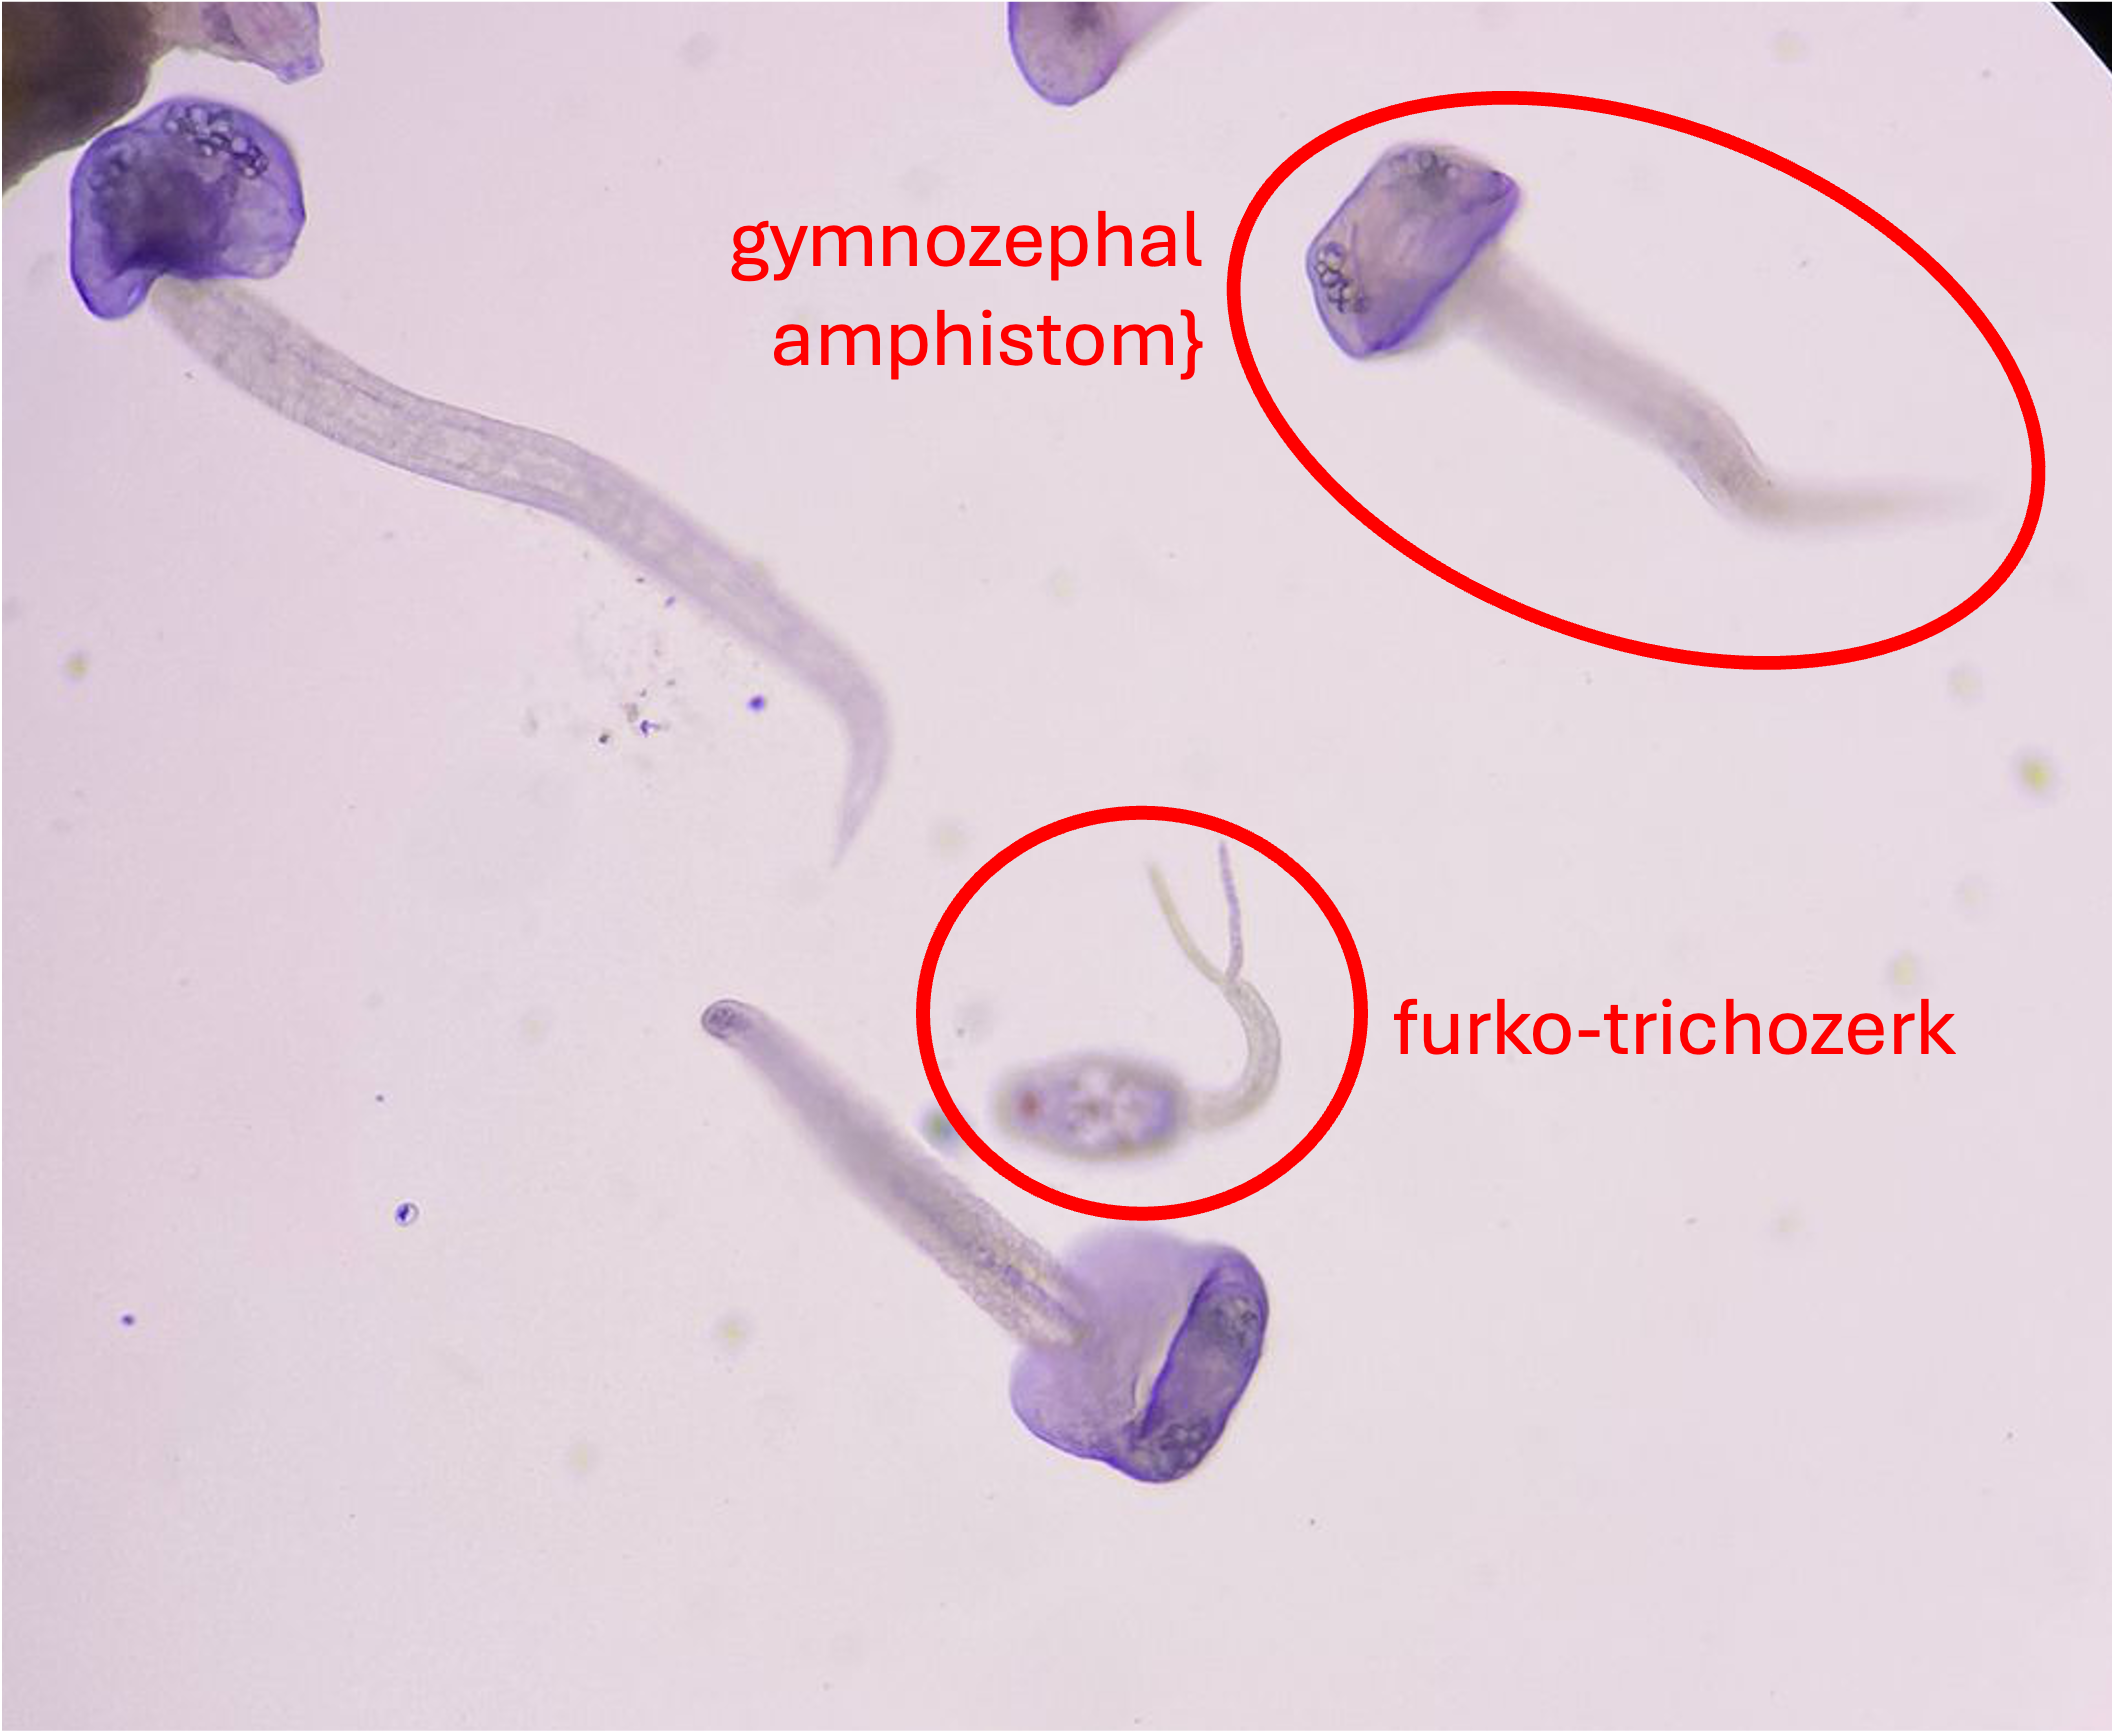
\includegraphics[width=\textwidth]{Zerkarien.png}
						\caption{Zerkarien}
						\label{fig: Zerkarien}
					\end{subfigure}
					\caption{Mikroskopische Aufnahme von Kommilitonen*innen der Larven der Spezies  Dicrocoelium dendriticum aus einer inifizierte Wasserschnecke. In \ref{fig:Redie} wurde die Larvenform Redie entdeckt und  in \ref{fig: Zerkarien} sind zwei Formen der Zerkarien zu sehen: gymnozephal amphistom und furko-trichozer}
					\label{fig: Trematodenlarven}
				\end{figure}
				
				Die Aufnahmen in Figure \ref{fig: Trematodenlarven} wurden von verschiedenen Komillitionen aufgenommen, da im vorliegende Präparat die Larvenstadien kaum erkennbar war (siehe Figure \ref{fig: crapTrematodenlarven}). Es wird vermutet, dass die Schnecken zu den Zeitpunkt viel zu lange tot waren, so dass auch der Parasit gestorben ist.
				
				\begin{figure}[H]
					\centering
					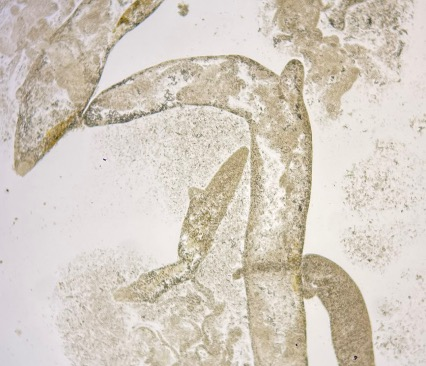
\includegraphics[scale=0.5]{Trematodenlarven.jpg}
					\caption{Mikroskopische Aufnahme der Larven der Spezies Dicrocoelium dendriticum aus einer infizierte Wasserschneck .}
					\label{fig: crapTrematodenlarven}
				\end{figure}
	
	\chapter{Apicomplexa}
		Apicomplexa sind einzellige eukaryotische Parasiten, die wie auch die Trematoden, in ihren Leben einen Generationswechsel und Wirtswechsel durchlaufen müssen.
		Die asexuelle Vermehrung beginng zuerst mit der Schizogonie, wo sich der Zellkern des Sporozoiten (haploides Genom) zuerst in in vielen Zellkernen teilt und dann der Cytoplasma sich in die einzelnen Zellen aufspaltet. Die einzelnen Zellen werden als Merozoiten bezeichnet. In der sexuelle Phase wandeln sich die Merozoiten in Gametozyten, die dann zu einer Zygoten verschmelzen. Aus dieser Zygoten entstehen durch die Meiose wieder haploide Sporozyten.\\
		Die bekanntesten Apicomplexa-Arten sind die Malaria-Erreger (Gattung: Plasmodium) und Toxoplasma gondii (Katzen-Parasit)\cite{wiki_apicomplexa}.
		
		\section{Giemsa-Färbung von Plasmodium in Humanblut}
			\subsection{Einleitung}
				Untersucht wird das mit Plasmodium falciparum infiziertes Humanblut.\\
				Dieser einzelliger Parasit ist der bekannteste Erreger der Gattung Plasmodium und ist der Auslöser für die tödliche tropische Krankheit Malaria tropica\cite{malaria}.
				Der Parasit bewirtet während seines Lebens die weibliche Stechmücke Anopheles, welches als Vektor fungiert und Menschen, welches als Endwirt fungiert, ab.\\
				Als Sporozoit wird der Parasit von der Mücke aufgenommen und wird durch einen Mückenstich auf dem MEnschen übertragen. Im menschlichen Blut erfolgt die Schizogonie (asexuelle Vermehrung). Hierbei wird zwischen der exoerythrozytär Schizogonie in den Leberzellen und  die erythrozytäre Schizogonie in den Erythrozyten unterschieden. 
				In den Erytrhorzyten entwickelt sich der Schizont zu Merozoiten und verursacht die typischen wellenartige Fieberschübe, die am Ende des Schizogonienentwicklung ausgelöst wird. Dieses Symptom wird ausgelöst, weil sich die die Schizonten sich in mehren Merozoiten teilt und dabei für die Freisetzung, den Erythrozyten zerstören.\\
				
				Die Differenzierung zu männlichen und weiblichen Gametozyten, findet nicht bei allen Merozoiten statt, die undifferenzierten Merozoiten können hier dann andere Erythrozytenzellen befallen, währen die Gametozyten wieder von der Anopheles Mücke aufgenommen wird und der Zyklus vom Neuem beginnt.\\
				In diesen Versuch wird die verschiedenen Stadien des Erregers untersucht und die Parasitämie bestimmt. 
				Die Parasitämie ist ein wichtiger Indikator, um zu beurteilen wie viele Erythrozyten infiziert wurden\cite{parasitämie}. Je nach Grad wird von einem unkomplizierten (1-5 $\%$) und komplizierten (mehr als $\%$) Malaria gesprochen\cite{malaria}.
			\subsection{Methode}
				Die vorgefertigten Blutaufstriche wurden für 10 Minuten mit Giemsa-Lösung (1:10 mit Wasser) gefärbt. Das Präparat wurde in Wasser gewaschen und bei 100-fache Vergrößerung (Immersionsöl) untersucht.
				
			\subsection{Ergebnis}
				In den meisten Erythrozyten befand sich der Parasit Plasmodien merizoitisches Ring (Figure \ref{fig:1}). Als zweithäufigsten waren die Erythrozyten mit Plasmodien infiziert, die sich in den frühen Schizontenstadien befanden (Figure \ref{fig:2}). Im Präparat wurde nur ein weiblichen Gametocyten entdeckt(Figure \ref{fig:3}).
				\begin{figure}[H]
					\centering
					\begin{subfigure}[b]{0.3\textwidth}
						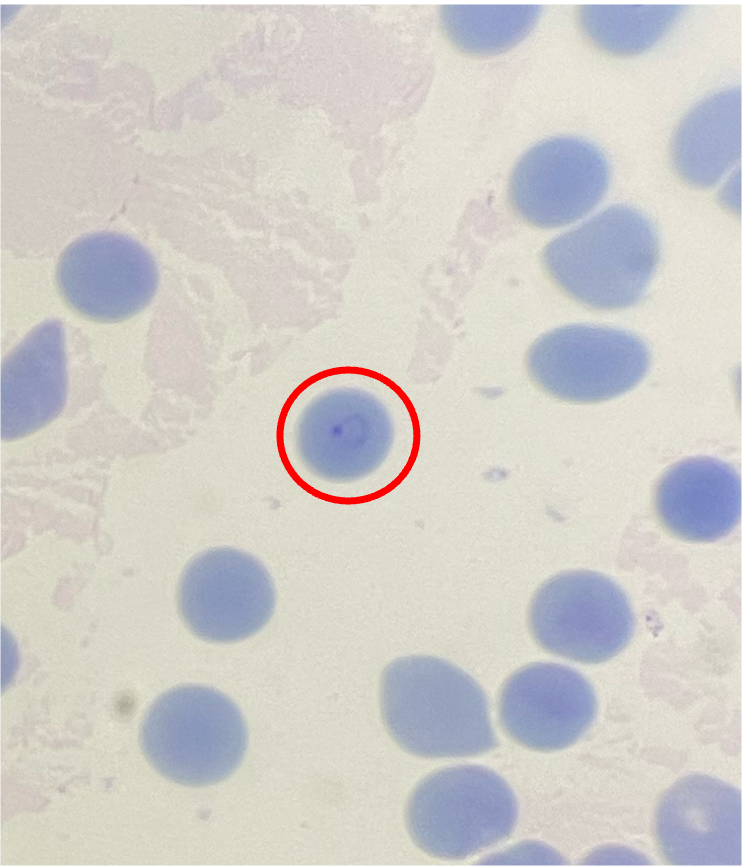
\includegraphics[width=\textwidth]{plas3.png}
						\caption{ringförmig}
						\label{fig:1}
					\end{subfigure}
					\hfill
					\begin{subfigure}[b]{0.3\textwidth}
						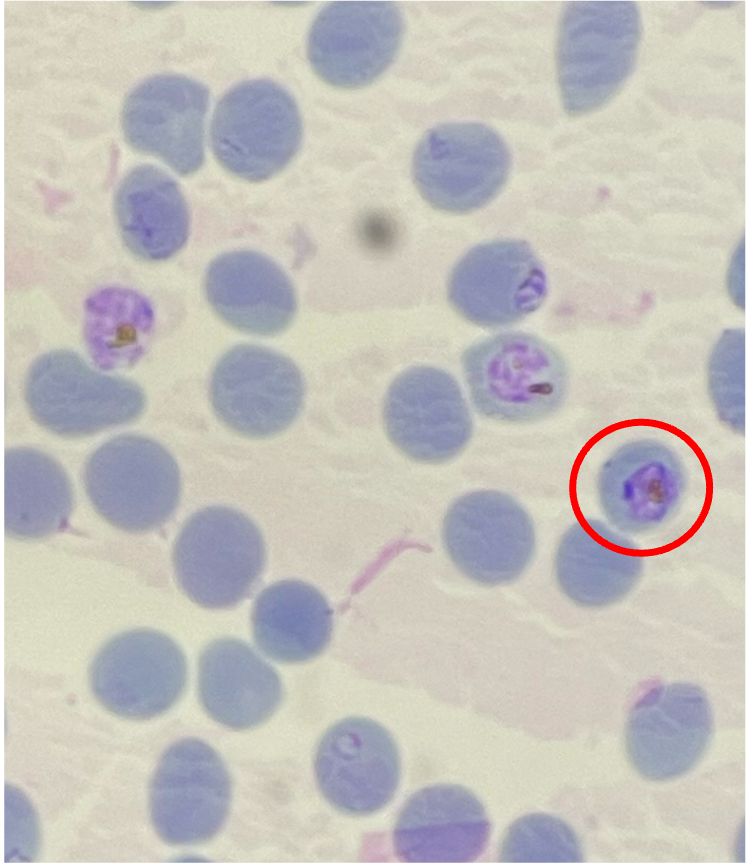
\includegraphics[width=\textwidth]{plas1.png}
						\caption{Frühstadium Schizont}
						\label{fig:2}
					\end{subfigure}
					\hfill
					\begin{subfigure}[b]{0.3\textwidth}
						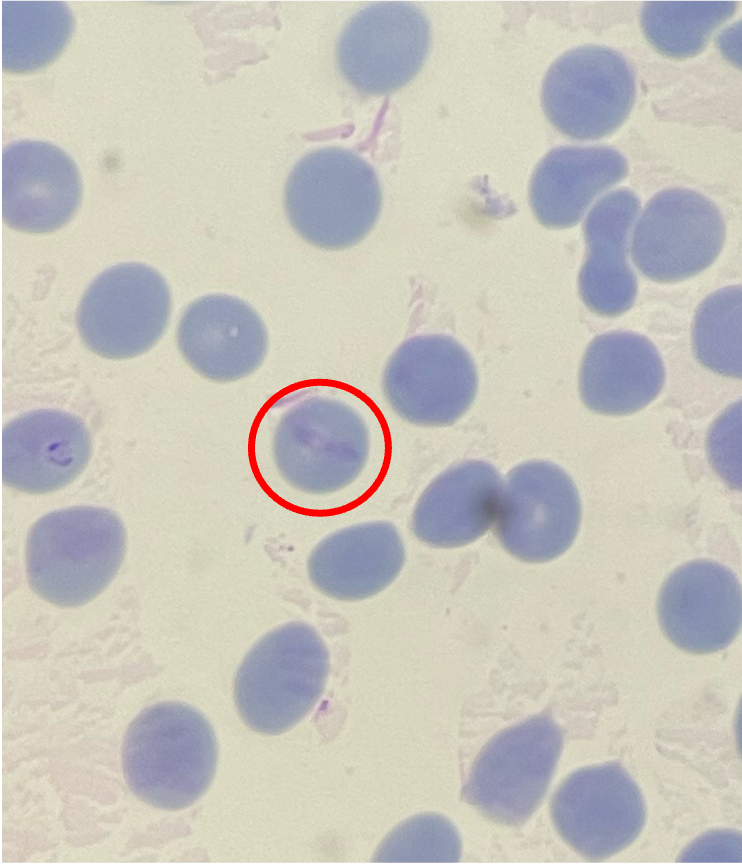
\includegraphics[width=\textwidth]{plas2.png}
						\caption{weiblicher Gametozyt}
						\label{fig:3}
					\end{subfigure}
					\caption{Giemsa-Färbung eines mit Plasmodium falciparum infiziertes Humanblutes. Der Parasit befand sich in unterschiedlichen metamorphologischen Stadien. In \ref{fig:1} befand sich der Erreger im Ringstadium, in \ref{fig:2} befindet sich der Erreger in der frühen Schizontenstadium und in \ref{fig:3} hat sich der Erreger in einem weiblichen Gametozyten entwickelt.}
					\label{fig: p_falciparum}
				\end{figure}
				
				Die Parasitämie wird nach der Gleichung \ref*{eq:Parasitämie} bestimmt.
				
				\begin{equation}\label{eq:Parasitämie}
					P_{\%} = \frac{\sum P \cdot 100 \%}{\overline{E} \cdot F}
				\end{equation}
				\\
				Dabei steht P für die Anzahl der infizierte Erythrozyten, $\overline{E}$ für die Anzahl der Erynthrozyten in einem Feld (Als repräsentative Zahl) und F für die Anzahl der Feldern.\\
				
				\begin{equation}\nonumber
					P_{\%} = \frac{64 \cdot 100 \%}{167 \cdot 10} = \underline{3.8 \%}
				\end{equation}
				\\
				Für das Präparat wurde eine Parasitämie von 3.8$\%$ bestimmt.
			\subsection{Diskussion}
				In den vorliegende Blutprobe wurde eine Parasitämie von 3.8$\%$ bestimmt.
				Der Durchschnittswert vom allen Blutpräparaten der Gruppe 4 (nachmittags) lag bei 3.9$\%$. 
				Der Wert kann vom wahren Wert etwas abweichen, da nicht alle Bereiche des Ausstriches homogen waren und nur von einem Feld die Erythrozyten gezählt wurden.\\
	
		\section{Gregarinenparasiten im Totenkopfschabe Blaberus craniifer}
			\subsection{Einleitung}
				Die Totenkopfschabe Blaberus craniifer wird oftmals als Futtertier für Terrarientiere genutzt und ist zudem ein Wirt des Parasiten Gregarnien, welches ebenfalls zu den Apicomplexa gehören.\\
				Als Oocysten werden die Parasiten über die Nahrung vom Wirt aufgenommen, wo die Sporozoiten im Wirt freigesetzt werden und sich zu Trophozoiten weiterentwickeln.
				Hier wechselt der Parasit von der asexuelle Vermehrung zu der sexuelle Vermehrung, wo die Trophozoiten zu Gamonten weiterentwickeln. \\
				In der sexuellen Fortpflanzung heften sich die weiblichen und männlichen Gregarien aneinander und bilden eine Zyste, die Gamontenzyste bezeichnet wird. Aus der Zysten gehen dann die Gameten hervor, die sich zu eine Zygote verschmelzen.\\
				Die Zygote bildet dann haploide Sporozoiten, die den Wirt verlassen und dann bei einer erneuten Nahrungsaufnahme mit ihren Lebenszyklus vom neuen beginnen\cite{Gregarinen}.\\
				\\
				Neben den Gregarine befallen auch andere Parasiten die Totenkopfschabe. \\
				Den Darminhaltes wird hier in diesen Versuch untersucht werden. Zudem wird die Schwimmgeschwindigkeit der Gregarnien untersucht und die Wirkung von Cytochalasin D auf die Motilität der Parasiten in den Totenkopfschabe.\\
				Cytochalasin D ist ein Aktininhibitor aus einem Pilzgift, das welches an Aktinfilamente bindet und somit die Polymerisation hemmt\cite{aktinhem}.
			\subsection{Methode}
				Darminhaltes des Totenkopfschabe Blaberus craniifer wird unterm Mikroskop charakterisiert.\\
				
				\subsubsection{Motilität des Gregarinen}
					Die Schwimmgeschwindigkeit des Gregarinen wird unterm Mikroskop bestimmt.\\
					Dann wird ein Tropfen 20 $\mu$M Cytochalasin D in Ringer-Lösung zu den Präparaten hinzugegeben und die Bewegung der Parasiten untersucht.\\
				
			
			\subsection{Ergebnis}
				\subsubsection{Parasiten in dem Darm des Blaberus craniifer}
					In Figure \ref{fig: Blaberus_darm} wurden zwei Parasitenarten gefunden, die Gregarinen (Figure \ref{fig:Apicomplexa}) und Ciliaten (Figure \ref{fig: Ciliaten}).
					Die Gregarine bewegen sich, anders als die Ciliaten, langsam und linear.
					\begin{figure}[H]
						\centering
						\begin{subfigure}[b]{0.46\textwidth}
							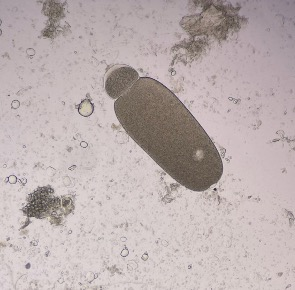
\includegraphics[width=\textwidth]{apicomplexa.jpg}
							\caption{Gregarinen, Apicomplexa}
							\label{fig:Apicomplexa}
						\end{subfigure}
						\hfill
						\begin{subfigure}[b]{0.5\textwidth}
							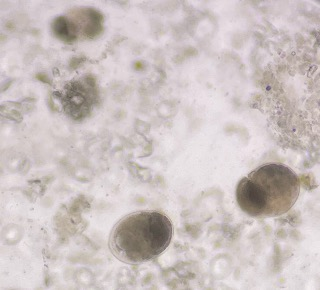
\includegraphics[width=\textwidth]{ciliaten.jpg}
							\caption{Ciliaten}
							\label{fig: Ciliaten}
						\end{subfigure}
						\caption{Darminhaltes des Totenkopfschabe (Blaberus craniifer). Es wurden zwei Arten gefunden, einmal eine Apicomplexa der Art Gregarinen \ref{fig:Apicomplexa} und Ciliaten \ref{fig: Ciliaten}}
						\label{fig: Blaberus_darm}
					\end{figure}
					
					

			\subsubsection{Untersuchung der Wirkung von Cytochalasin D auf die Motilität von Gregarinen}
				Die Die Geschwindigkeit des Gregarine wurde nach Gleichung \ref{eq: geschwindigkeit} bestimmt. Der Durchmesser des Sichtfeldes vom Okular betrug 2mm. Auf dem Photo wurde ein Durchmesser von 7.5 cm gemessen und wo der Parasit 7 mm innerhalb von 147 Sekunden geschwommen ist. Durch einen einfachen Dreisatz in Gleichung \ref{eq: dreisatz} wurde eine Strecke im Präparat, die der Parasit zurückgelegt hat, von 0.186 mm ermittelt.\\
				Die Geschwindigkeit betrug 1.26$\mu$m/s
				
				\begin{equation}\label{eq: geschwindigkeit}
					v = \frac{\text{zurückgelegte Strecke}}{\text{Zeit}}
				\end{equation}
				\\
				\begin{equation}\label{eq: dreisatz}
					\begin{split}
						2 mm &\quad\widehat{=}\quad s\\
						75 mm  &\quad\widehat{=}\quad 7 mm
					\end{split}
				\end{equation}
				
				\begin{figure}[H]
					\centering
					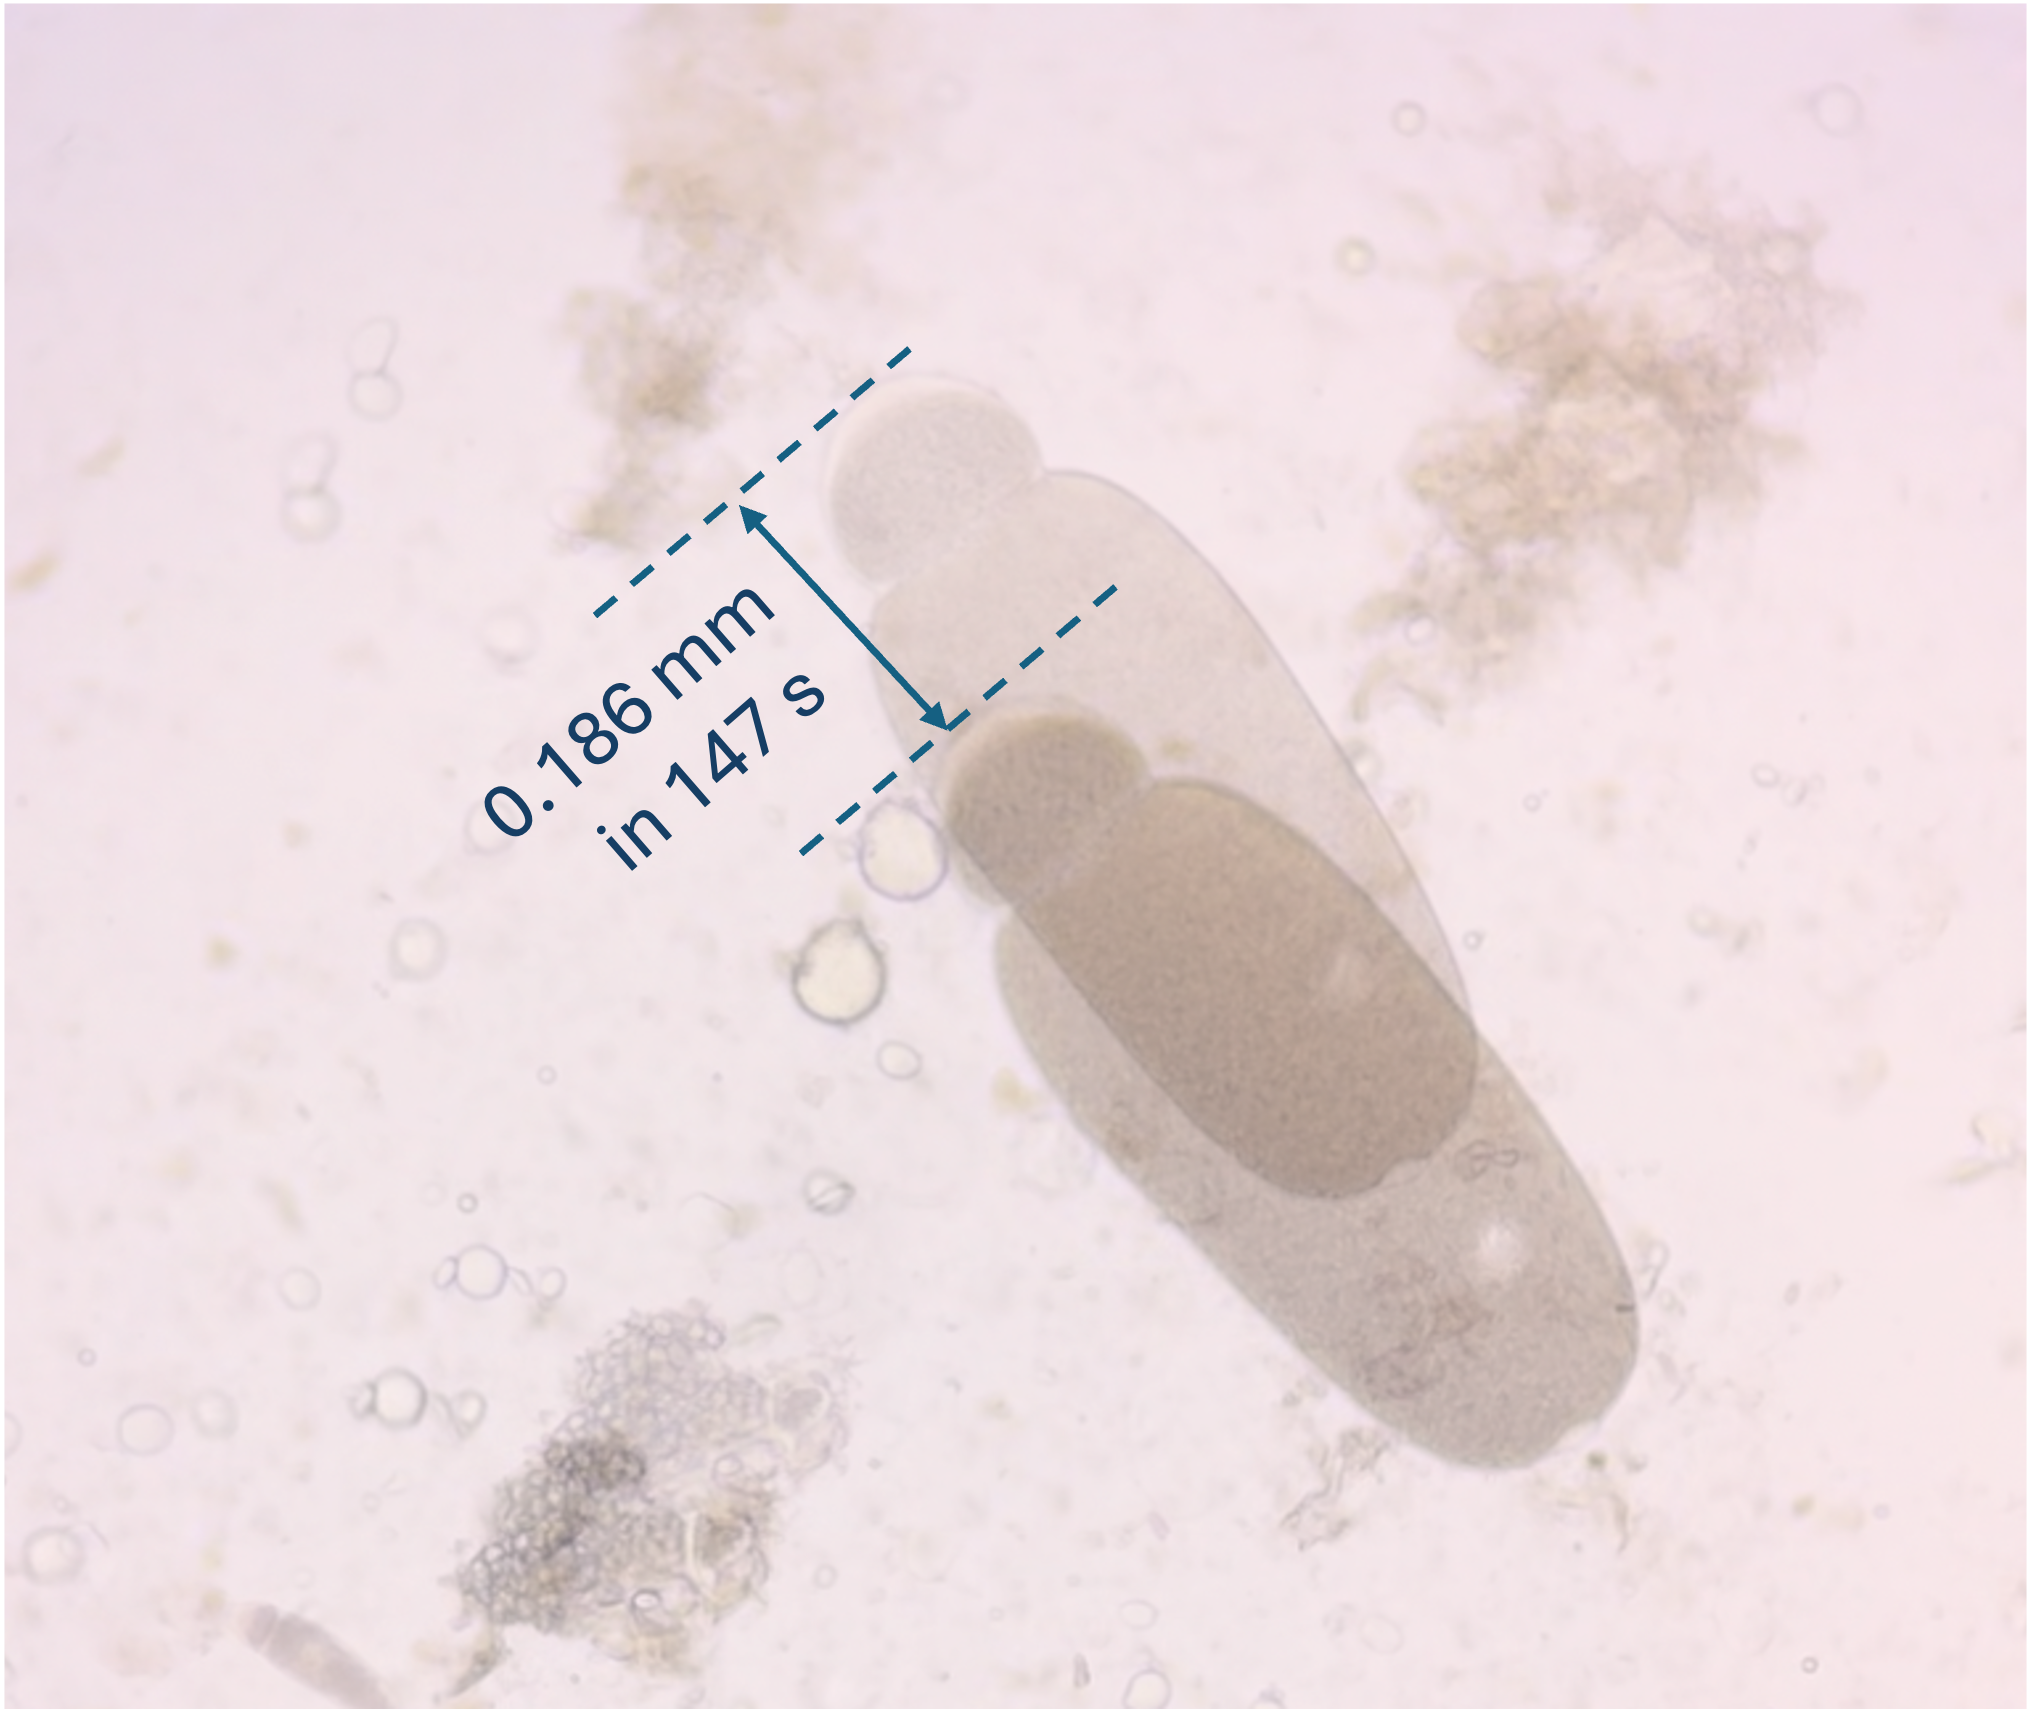
\includegraphics[scale=0.7]{apicomplexa_geschwindigkeit.png}
					\caption{Hinterlegte Strecke des Gregarinen-Parasiten in einem Zeitraum von 147 Sekunden. Die Geschwindigkeit beträgt 1.26$\mu$m/s. Isoliert wurde das Parasit aus dem Totenkopfschabe Blaberus craniifer.}
					\label{fig: natives Apicomplexabewegung}
				\end{figure}
				
				In Table \ref{tab: aktinhem} wurde die Mobilität der beiden Parasitenarten vor und nach der Zugabe vom Aktimhemmer Cytochalasin D dargestellt. Die Gregarinen waren nach der Zugabe immobil.
				\begin{table}[H]
					\centering
					\caption{Bewegung der Parasiten des Darminhaltes vor und nach der Zugabe von einem Tropfen Cytochalasin D.}
					\label{tab: aktinhem}
					\begin{tabular}{ccc}
						\toprule
						&Gregarinen & Ciliaten\\
						\midrule
						ohne Cytochalasin D & mobil & mobil \\
						mit Cytochalasin D & immobil & mobil\\
						\bottomrule			
					\end{tabular}
				\end{table}
				
			\subsection{Diskussion}
			Der Darminhaltes des Blaberus craniifer war mit den Parasiten der Art Gregarinen und Ciliaten infiziert (siehe Figure \ref{fig: Blaberus_darm}).\\
			Die Geschwindigkeit des Gregarinen betrug im Präparat 1.26$\mu$m/s. Nach der Zugabe von Cytochalasin D wurde keine Bewegung von Gregarinen festgestellt, während die Ciliaten sich noch bewegt haben.\\
			Es kann davon ausgegangen werden, dass die Bewegung von den Gregarinen aktinabhängig sind und vom Ciliaten nicht.
	
	
	\chapter{Anhang}
		\section{PCR}
		\begin{table}[H]
			\centering
			\caption{MasterMix Pipettierschema für 3 PCR-Raktionen. Der MasterMix ist 3-Fach konzentriert}
			\label{tab: Mastermix-Pipettierschema}
			\begin{tabular}{cc}
				\toprule
				& Volumen in $\mu$L\\
				\midrule
				10x Reaktionspuffer & 7.5 \\
				Oligo for & 1.5\\
				Oligo rev & 1.5\\
				dNTP Mix & 1.5\\
				Taq Polymerase & 0.3\\
				H$_2$O & 57\\
				\bottomrule
			\end{tabular}
		\end{table}
		
		\begin{table}[H]
			\centering
			\caption{PCR-Cyclus Einstellungsprogramm. 34 Cyclen wurde durchgeführt.}
			\label{tab: PCR-Cyclen}
			\begin{tabular}{cc}
				\toprule
				94°C & 3 Minute\\
				94°C & 45 Sekunde\\
				48°C & 45 Sekunde\\
				72°C & 1 Minute\\
				72°C & 5 Minute\\
				4°C & unendlich\\
				\bottomrule
			\end{tabular}
		\end{table}
		
		\begin{table}[H]
			\centering
			\caption{Sequenz vom Forward- und Reverse-Primer für die PCR. Folmer (1994).}
			\label{tab: Primer}
			\begin{tabular}{cc}
				Forward & 5’ GGTCAACAAATCATAAAGATATTGG 3'\\
				Reverse & 5’ TAAACTTCAGGGTGACCAAAAAATCA 3’\\				
			\end{tabular}
		\end{table}
		
		
		\begin{table}[H]
			\centering
			\caption{Consencus-Referenzsequenz vom anderen morphologischen Tier, die vom Betreuer zur Verfügung gestellt wurde.}
			\label{tab: Vergleichssequenz}
			\begin{tabular}{l}
				TTTTAGGGGCCTGATCAGCTATAGCTGGTACAGGCATAAGAGTACTAATTCGAATTGAAT\\
				TAGCTCAACCCGGCACATTTCTAGGAAATGATCAAATTTATAATACTATTGTAACCGCAC\\
				ATGGATTAGTAATAATCTTCTTTATAGTAATACCTATTTTAATTGGAGGATTTGGTAATT\\
				GGTTAATTCCATTAATAATTGGGGCCCCAGATATAGCATTTCCGCGACTTAATAATCTAA\\
				GATTCTGACTACTTCCACCATCCATAATTATACTAGTATTCTCTGCATTTGTAGAAAATG\\
				GAGTAGGTACTGGATGAACAGTATACCCTCCTCTAGCATACAATATTGCACACTCTGGCC\\
				CATCTGTAGATATAGCTATCTTCTCATTACATTTAGCGGGAGCATCATCTATCCTAGGGT\\
				CCCTAAATTTTATTTCAACTGTAGCTAATATACGATGAAAAGGAATAACTATAGATCGAA\\
				TTCCTTTATTTATTTGATCAGTAATTATTACTACAGTTCTTTTACTACTCTCCTTACCTG\\
				TACTAGCAGCAGCAATTACAATATTATTAACTGATCGAAACCTAAATACATCATTCTTTG\\
				ACCCAGCAGGTGGAGGAGATCCTATTTTATTCCAACACTTATTTTGATTTTTTG\\
			\end{tabular}
		\end{table}
		
		\section{Anatomische Zeichnung Regenwurm und Medizinischer Egel}
		\begin{figure}[H]
			\centering
			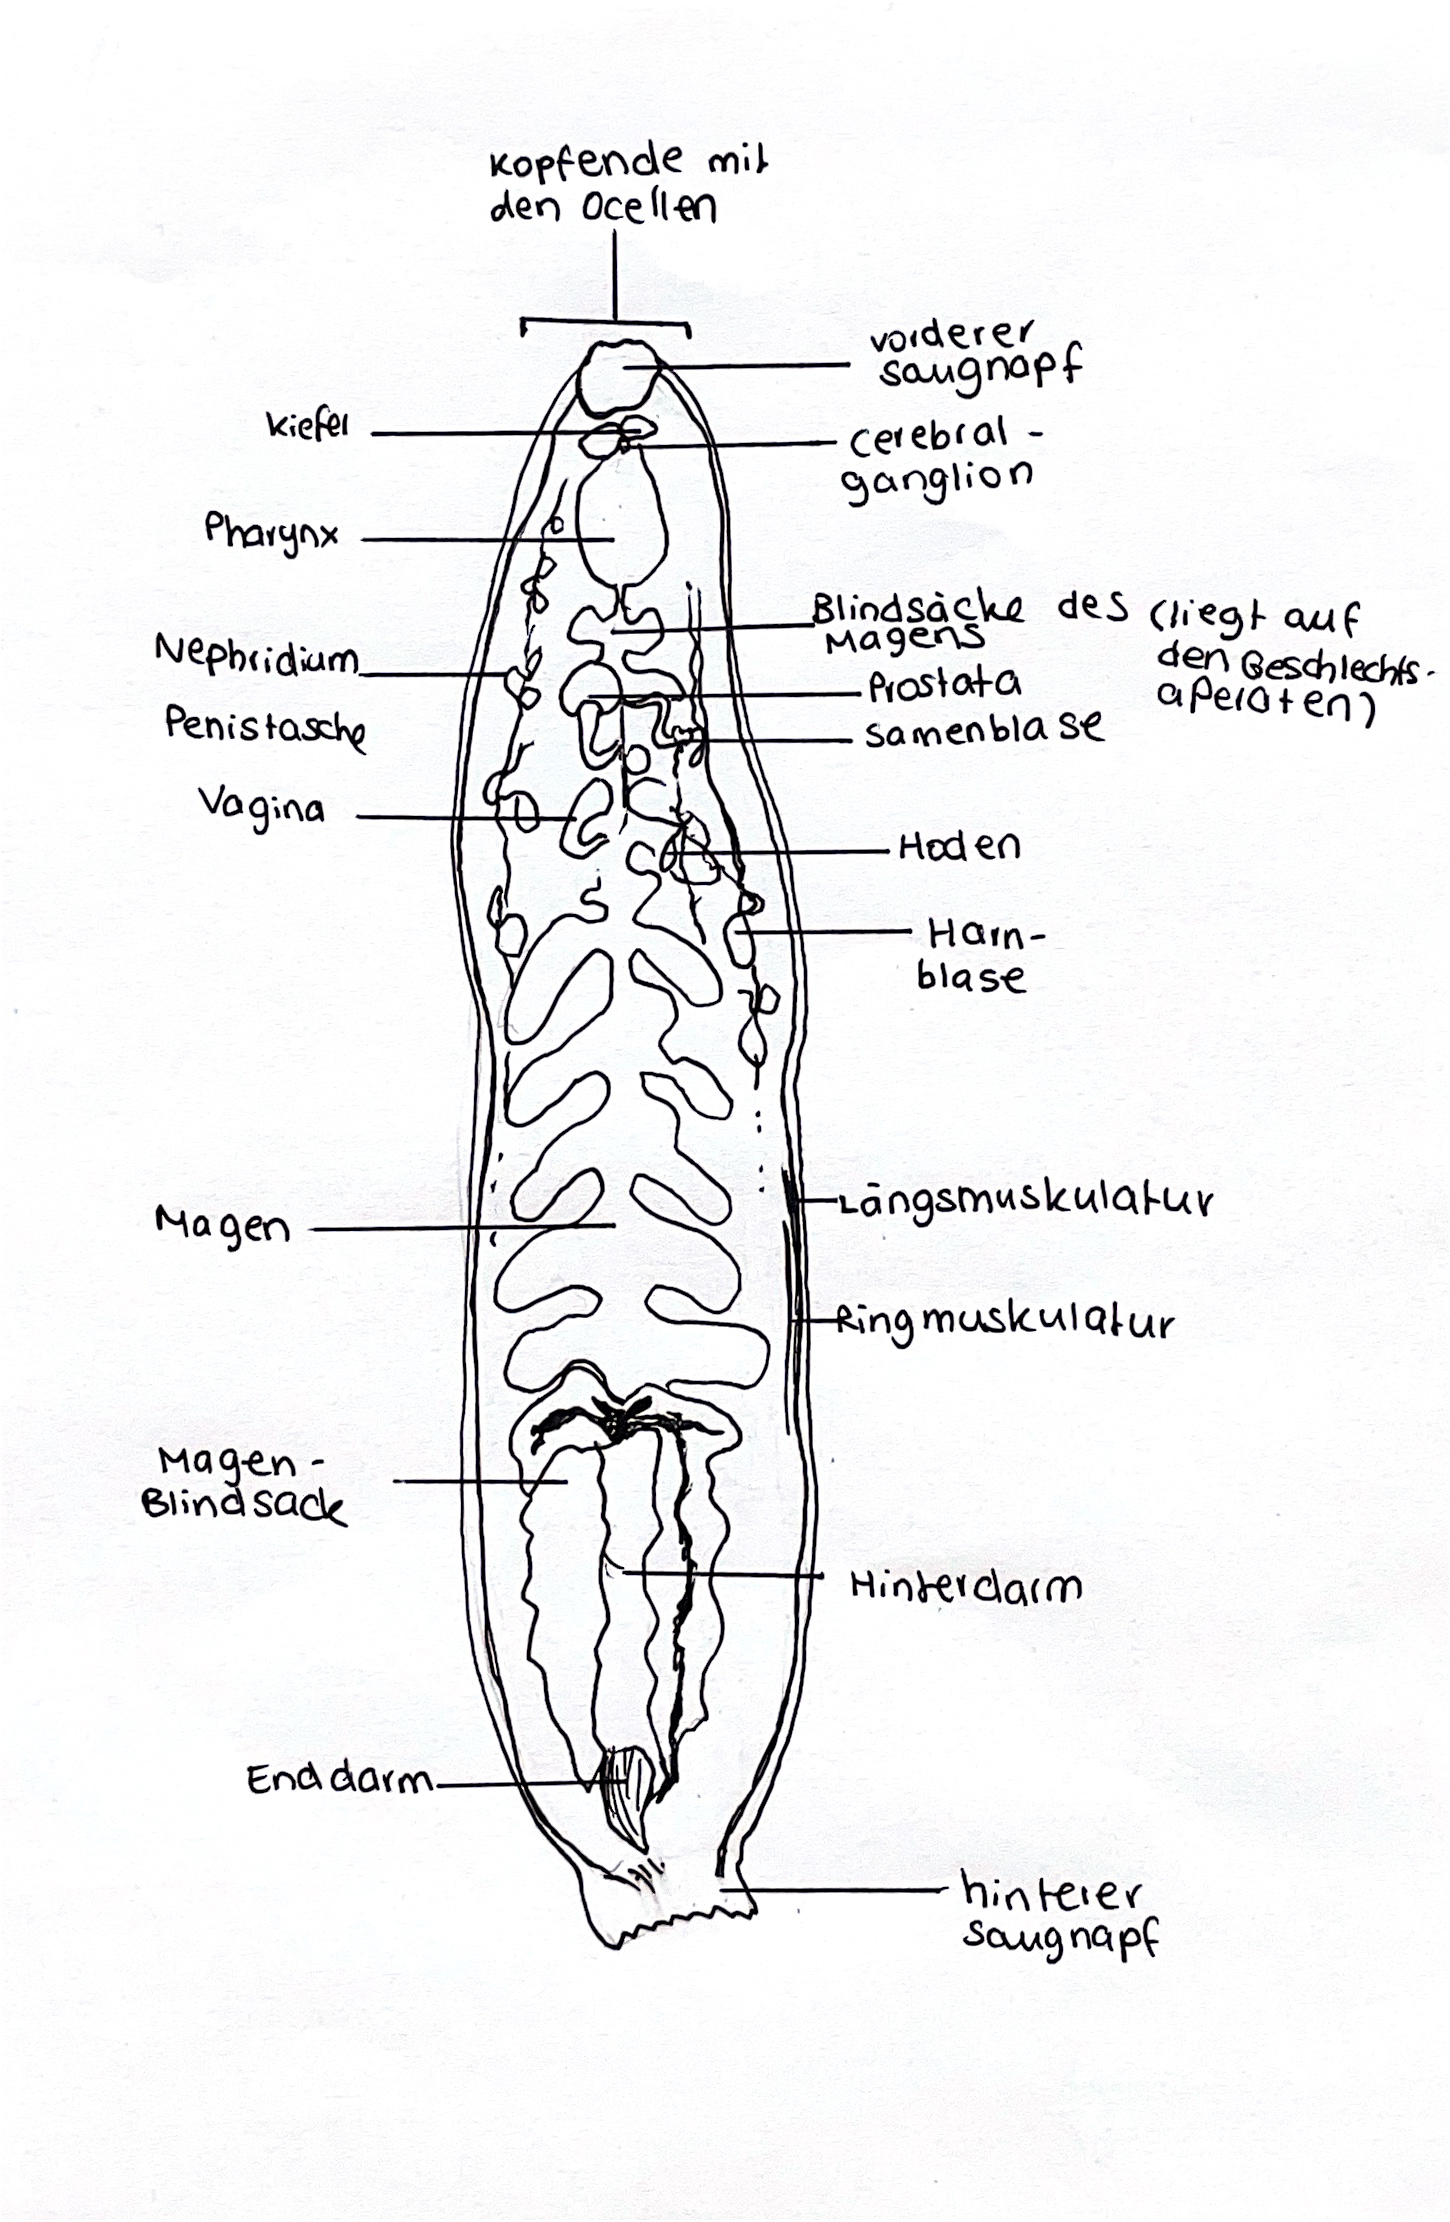
\includegraphics[scale=0.25]{Egel.JPG}
			\caption{Anatomische Skizze des Medizinischen Egels (Hirudo verbana)}
			\label{fig:Egel_ana}
		\end{figure}
		
		\begin{figure}[H]
			\centering
			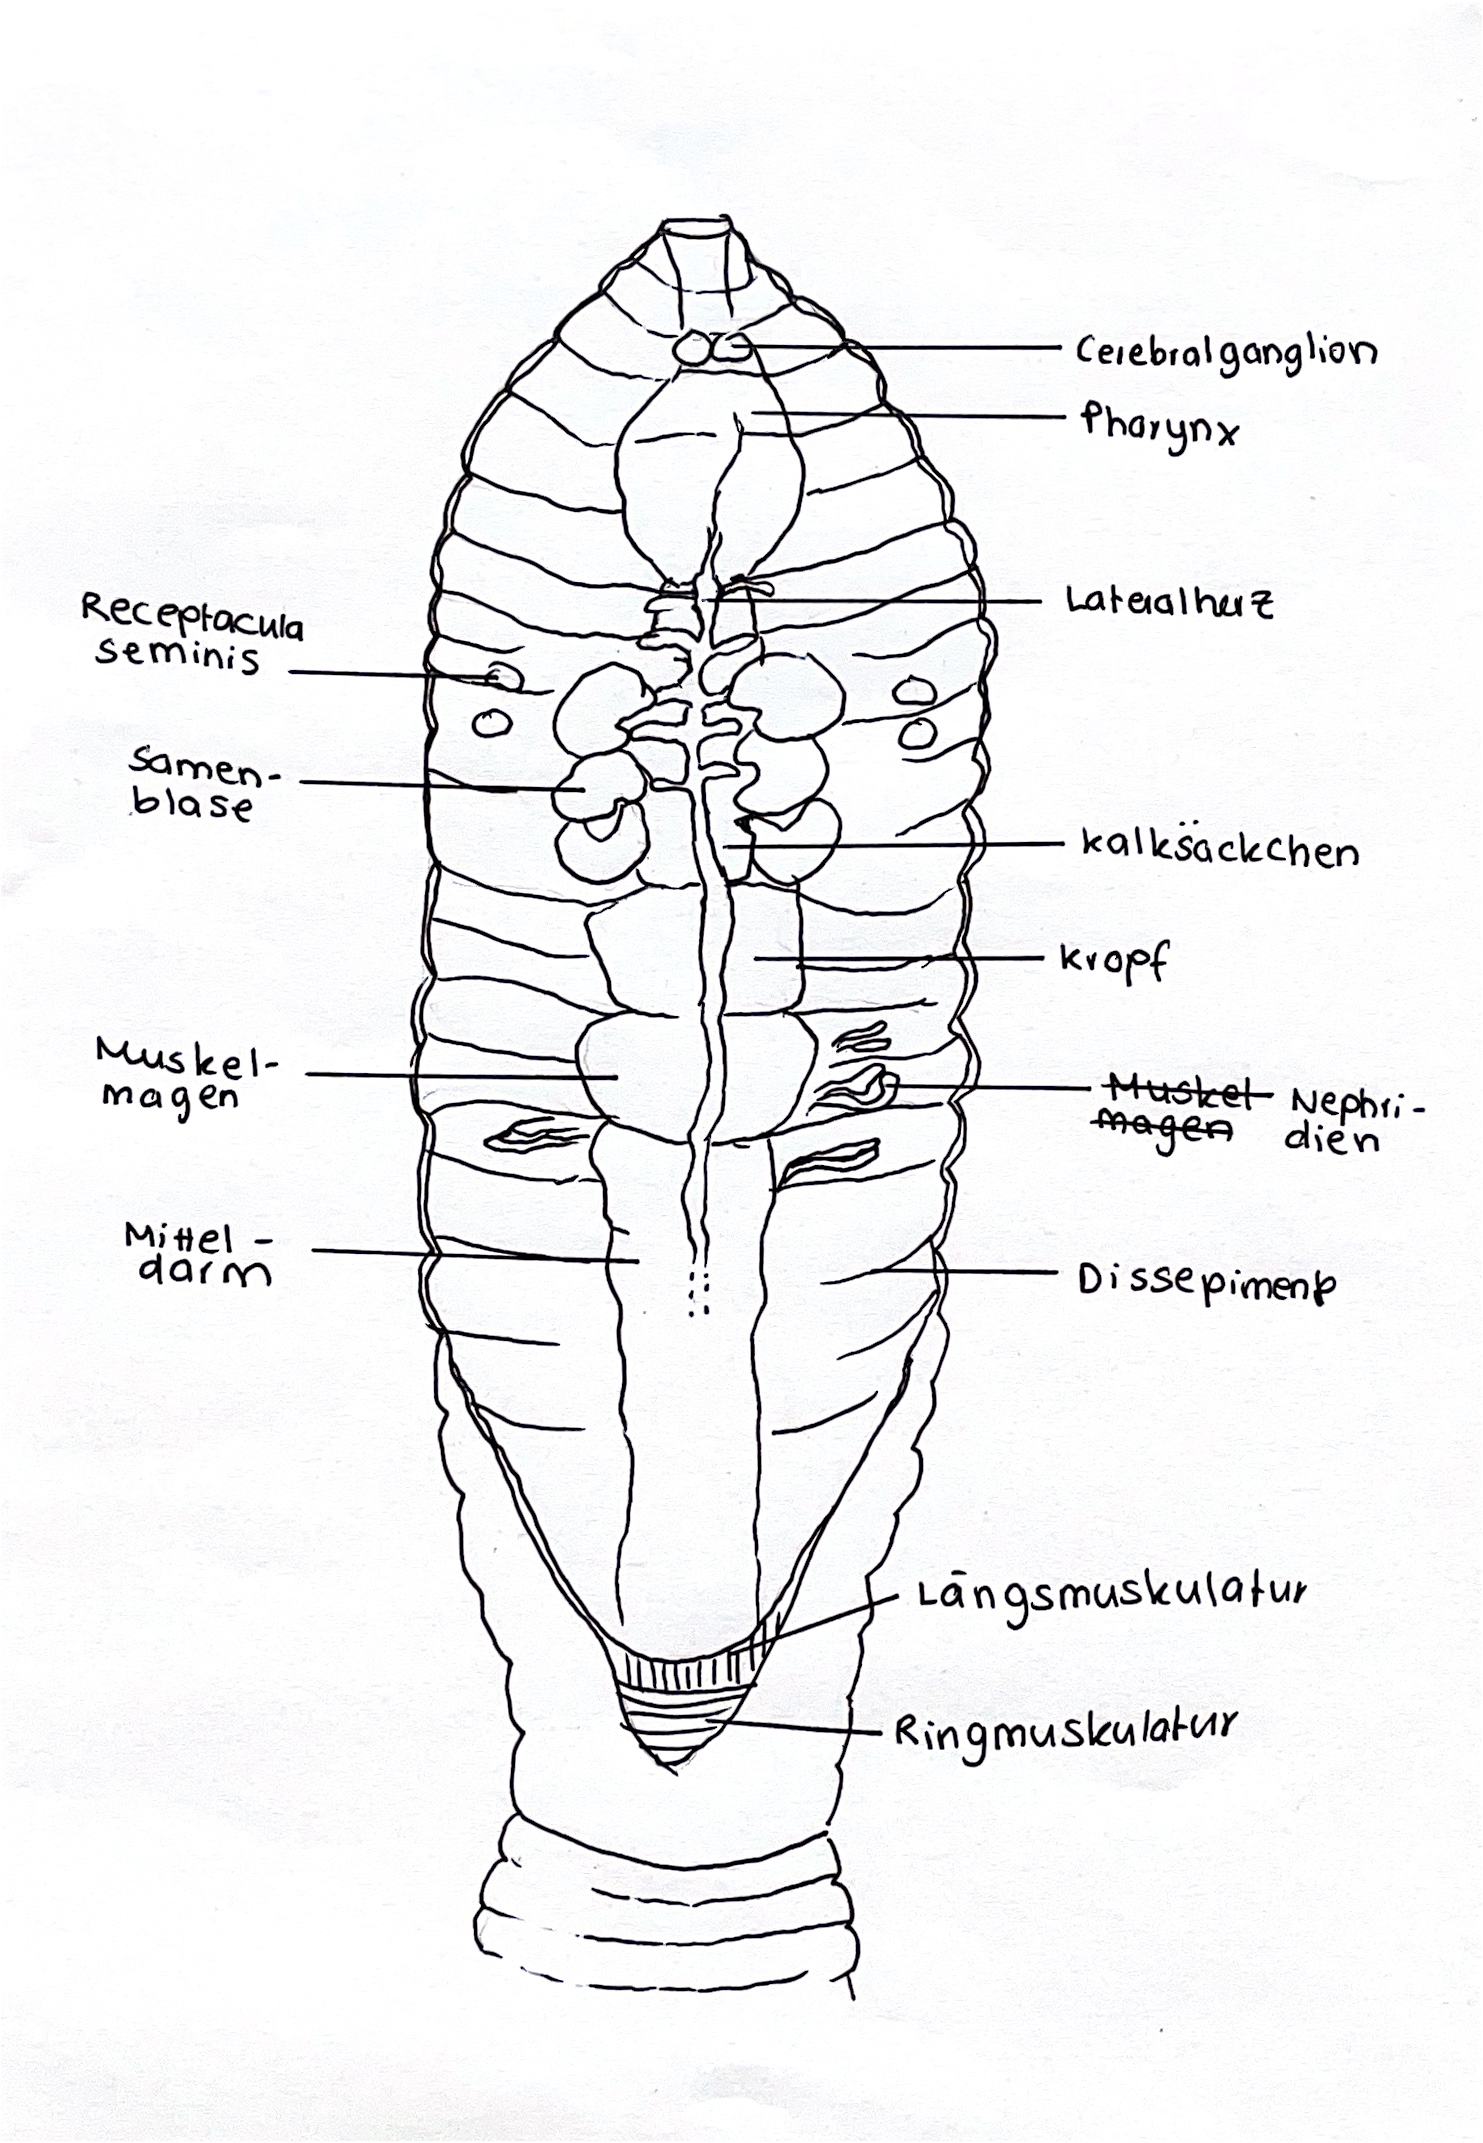
\includegraphics[scale=0.25]{Regenwurm.JPG}
			\caption{Anatomische Skizze des Regenwurmes (Limbricus terrestris)}
			\label{fig:Regenwurm_ana}
		\end{figure}
		
		\section{Plasmodium in Erythrozyten}
				\begin{table}[H]
				\centering
				\caption{Anzahl von Parasiten in den Erythrozyten in 10 verschiedenen Feldern, um die Parasitämie zu bestimmen.}
				\label{tab: Eryzahl}
				\begin{tabular}{cc}
					\toprule
					Feldernummer & Anzahl Plasmodium in den Erythrozyten\\
					\midrule
					1 & 6 \\
					2 & 7 \\
					3 & 5 \\
					4 & 8 \\
					5 & 8 \\
					6 & 7 \\
					7 & 9 \\
					8 & 6 \\
					9 & 5 \\
					10 & 3 \\
					\bottomrule			
				\end{tabular}
			\end{table}
		
		
		
		
	\addcontentsline{toc}{section}{Bibliography}
	\bibliographystyle{plainurl}
	\nocite{*}
	\bibliography{Literatur}
	\newpage
\end{document}